\documentclass[12pt]{article}

\usepackage[margin=50pt]{geometry}
\usepackage{amsmath}
\usepackage{amssymb}
\usepackage{graphicx}
\usepackage{csquotes}
\usepackage{array}
\usepackage{caption}
\usepackage{diagbox}
\usepackage{hyperref}

\graphicspath{/images}
\geometry{footskip=0.8cm}

\newlength{\Oldarrayrulewidth}
\newcommand{\Cline}[2]{%
  \noalign{\global\setlength{\Oldarrayrulewidth}{\arrayrulewidth}}%
  \noalign{\global\setlength{\arrayrulewidth}{#1}}\cline{#2}%
  \noalign{\global\setlength{\arrayrulewidth}{\Oldarrayrulewidth}}
}

\newcommand\Thickvrule[1]{%
  \multicolumn{1}{!{\vrule width 2pt}c!{\vrule width 2pt}}{#1}%
}

\title{\vspace{-1.0cm}Game Theory}
\author{Thomas Vroom}

\begin{document}
\maketitle

\tableofcontents

%
% Topic 1 - A Bankruptcy Problem from the Talmud
%
\newpage
\section{A Bankruptcy Problem from the Talmud}
In the Babylonian Talmud, which is a collection of Jewish religious and legal decisions laid down during the first five centuries A.D., the following \textit{Mishna} can be found:

\begin{displayquote}
    "If a man who was married to three wives died and one was owed 100, the other 200, and the third 300, and the estate was worth only 100, then the sum is divided equally.

    If the estate was worth 200 then the claimant of 100 receives 50 and the claimants respectively of 200 and 300 each receive 75.

    If the estate was worth 300 then the claimant of 100 receives 50, the claimant of 200 receives 100 and the claimant of 300 receives 150.

    Similarly, other profits or losses have to be shared in the same manner."
\end{displayquote}

\noindent
This information can be summarized into a table, called the \textbf{Talmud table:}

\begin{figure}[h]
    \centering
    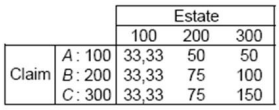
\includegraphics[scale=1.2]{images/TalmudTable.PNG}
    \caption{The Talmud table.}
\end{figure}

\noindent
In the 20th century game theorists discovered that all numbers in the Talmud table correspond exactly to the \textbf{nucleolus} of so-called \textbf{cooperative games} (chapter 2).
However, the field of game theory was only established in the second half of the twentieth century.
Besides, a study of historic documents showed that among Talmudic scholars the meaning and origin of the numbers in the table were a mystery for nearly 2000 years.
In finding the fundamental link between the Talmud table and game theory, game theorists found another Mishna to play a central role in understanding the numbers of the table.

\subsection{Contested Garment Problem}
The following Mishna can also be found in the Babylonian Talmud:

\begin{displayquote}
    "Two hold a garment; one claims it all, the other claims half.
    
    Then the one is awarded $\frac{3}{4}$, the other $\frac{1}{4}$."
\end{displayquote}

\noindent
We can visualize this \textbf{contested garment problem} by a rectangle in which one person $(A)$ claims the full rectangle, while the other $(B)$ just claims the right-side half of it:

\begin{figure}[h!]
    \centering
    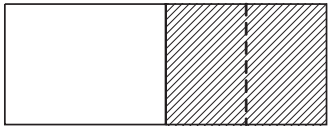
\includegraphics{images/CGexample1.PNG}
\end{figure}

\newpage
\noindent
In reality, these people are only fighting over the shaded part of the rectangle.
Person $B$ has no problem with person $A$ claiming the left-side half of the rectangle.
The Mishna says that the part both people are claiming should be divided equally.
As such, the dotted line marks the division rule, which says that $\frac{3}{4}$ should go to $A$ and $\frac{1}{4}$ should go to $B$.

\noindent
\\
Following similar reasoning, we can find that all numbers in the Talmud table are supported by the contested garment principle.
We therefore say that the numbers in Talmud table are \textbf{consistent} with the contested garment principle.
Since the Mishna says that other amounts have to be shared "in the same manner", it means we always have to find a solution that is \textbf{CG-consistent}.

\noindent
\\
To share an amount of 250 among three people $A, B, C$ claiming 100, 200 and 300 respectively, we have to find a solution $(a, b, c)$ with properties:

\begin{enumerate}
    \item $a + b + c = 250$;
    \item for $A$ and $B$ the CG-solution for sharing $a + b$ is $(a, b)$;
    \item for $B$ and $C$ the CG-solution for sharing $b + c$ is $(b, c)$;
    \item for $A$ and $C$ the CG-solution for sharing $a + c$ is $(a, c)$.
\end{enumerate}

\noindent
This can be quite a puzzle to figure out, but luckily there exists a sequential procedure to solve any bankruptcy problem for the CG-consistent solution.
This is called the \textbf{coalition procedure}.

\subsection{The Coalition Procedure}
In the cases where there is either 200 or 300 to be shared, widows $B$ and $C$ are acting as a coalition claiming 500 against widow $A$ (who is claiming 100).
Under these circumstances the CG-solution for sharing 200 would yield 150 for the coalition and 50 for widow $A$.
Next, widows $B$ and $C$ share the 150 according to the CG-principle, where each of them gets 75.
Similarly, one can derive the solution $(50, 100, 150)$ for the 300 case.

\noindent
\\
However, if we were to use this procedure for the 100 case, then again widow $A$ receives 50, but $B$ and $C$ are getting 50 together as well and would share it half-half.
The final result would be $(50, 25, 25)$ and $A$ claiming the least would get the most.
This is clearly not CG-consistent, so in the coalition procedure we have to be careful that members of the coalition are not getting less than the person with a lower claim.

\noindent
\\
The coalition procedure allows us to easily scale the bankruptcy problem to any number of widows.
Take for example a 5-person bankruptcy problem denoted by:

\[ (400 \text{ } | \text{ } 100, 160, 250, 300, 350) \]

\noindent
Here an estate of $E = 400$ has to be shared among five widows, claimants $C_1, C_2, C_3, C_4, C_5$ who claim $c_1 = 100, c_2 = 160, c_3 = 250, c_4 = 300, c_5 = 350$ respectively.
While going through the procedure we have to keep in mind that claimants claiming less should get less.
This means we expect a solution $(x_1, x_2, x_3, x_4, x_5)$ where $x_5 \geq x_4 \geq x_3 \geq x_2 \geq x_1$.

\newpage
\noindent
We can solve this bankruptcy problems using the following steps:

\begin{enumerate}
    \item We first group claimants $C_2, C_3, C_4$ and $C_5$ to be one widow, $W_1$, who claims $c_2 + c_3 + c_4 + c_5 = 1060$, while $C_1$ is still claiming $c_1 = 100$.
    When $C_1$ and $W_1$ share the estate $E = 400$ according to the CG-principle, $C_1$ receives $x_1 = 50$ and $W_1$ receives $E_1 = 350$. 
    \item Now we share 350 among widows $C_2$, claiming $c_2 = 160$, and $W_2$, claiming $c_3 + c_4 + c_5 = 900$.
    The CG-solution gives $x_2 = 80$ for $C_2$ and $E_2 = 270$ for $W_2$.
    \item The remaining 270 is now to be shared among $C_3$ claiming $c_3 = 250$ and $W_3$ claiming $c_4 + c_5 = 650$.
    The CG-solution for this would be to give 125 to $C_3$ and 145 to $W_3$.
    However, this would imply that either $C_4$ or $C_5$ is getting less than $C_3$, which would contradict the CG-principle.
    Therefore, $C_3, C_4$ and $C_5$ should share the amount 270 equally, which gives $x_3 = x_4 = x_5 = 90$.
\end{enumerate}

\noindent
The procedure ends and the estate of 400 is shared among the widows as $(50, 80, 90, 90, 90)$.

\noindent
\\
To verify that this solution is indeed CG-consistent, we have to check that for every pair of claimants $(C_i, C_j)$ involved in a problem to share $x_i + x_j$, the CG-solution would be $(x_i, x_j)$.
Although this holds for the example above, the procedure is not fully developed yet.

\noindent
\\
Say we are given a 3-person bankruptcy problem $(200 \text{ } | \text{ } 100, 110, 120)$.
In step 1 we have $C_1$ with a claim of 100 against $W_1$ with a claim of 230.
The CG-solution for this would be $(50, 150)$.
Next, 150 would be shared among $C_2$ and $C_3$ as the CG-solution $(70, 80)$.
Thus, the final solution would be $(50, 70, 80)$.
However, this solution is not CG-consistent, because the CG-solution for $C_1$ and $C_2$ sharing $50 + 70 = 120$ is $(55, 65)$.
What went wrong?
If we examine the solution $(50, 70, 80)$ provided by the procedure, then we observe that claimant $C_1$ loses 50 in view of their claim, while claimants $C_2$ and $C_3$ lose 40 each.
This brings us to the second issue we have to control in the procedure:
A claimant with a lower claim should never lose more than a claimant with a higher claim.
In general, for claims $c_1 \leq c_2 \leq ... \leq c_n$ we want to have a solution $(x_1, x_2, ... , x_n)$ with:

\begin{enumerate}
    \item $x_1 \leq x_2 \leq ... \leq x_n$ (no claimant gets less than a smaller claimant);
    \item $c_1 - x_1 \leq c_2 - x_2 \leq ... \leq c_n - x_n$ (no claimant loses more than a smaller claimant).
\end{enumerate}

\subsection{General Solution for the Bankruptcy Problem}
A bankruptcy problem is denoted as:

\[ (E \text{ } | \text{ } c_1, c_2, ... , c_n) \]

\noindent
Where an estate $E$ has to be shared among claimants $C_1, C_2, ... , C_n$ who claim amounts $c_1 \leq c_2 \leq ... \leq c_n$.
We assume that $E$ is non-negative and that the total claim $c_1 + c_2 + ... + c_n > E$.
We call a solution $(x_1, x_2, ... , x_n)$ to be \textbf{order preserving} if:

\begin{enumerate}
    \item $x_1 \leq x_2 \leq ... \leq x_n$ (no claimant gets less than a smaller claimant);
    \item $c_1 - x_1 \leq c_2 - x_2 \leq ... \leq c_n - x_n$ (no claimant loses more than a smaller claimant).
\end{enumerate}

\noindent
We can share the amount $E$ step by step among claimants $C_1, C_2, ... , C_n$ by taking in each step the smallest remaining claimant against a coalition of all bigger claimants.
Each step the small, individual player receives their share according to the 2-person CG-solution, as long as the order of the full solution $(x_1, x_2, ... , x_n)$ is preserved.

\newpage
\noindent
More precisely, if at step $i$ the remaining $n - i + 1$ claimants are $C_i$ and $\{C_{i + 1}, ... , C_n\}$, and the remaining estate is $E_i$, then:

\begin{enumerate}
    \item If
    \[ \frac{c_i}{2} \leq \frac{E_i}{n - i + 1} \leq \frac{c_i + c_{i + 1} + ... + c_n}{n - i + 1} - \frac{c_i}{2} \]
    Then give $\frac{c_i}{2}$ to claimant $C_i$ and continue with step $i + 1$.
    \item If
    \[ \frac{c_i}{2} \geq \frac{E_i}{n - i + 1} \]
    Then $E_i$ is equally divided under the remaining claimants.
    \item If
    \[ \frac{E_i}{n - i + 1} \geq \frac{c_i + c_{i + 1} + ... + c_n}{n - i + 1} - \frac{c_i}{2} \]
    Then the total debt $c_i + c_{i + 1} + ... + c_n - E_i$ gets equally divided under the remaining claimants (i.e. it is subtracted from their claim $c_j$).
\end{enumerate}

\noindent
It has been proven that this coalition procedure always leads to the GC-consistent solution.
It has also been shown that this procedure is \textbf{self-dual}, meaning gains and losses are treated in the same way.

\subsection{Communicating Vessels}
Another way to visualize the solution of a bankruptcy problem is using \textbf{communicating vessels}:

\begin{figure}[h]
    \centering
    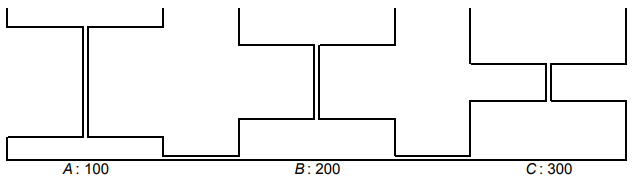
\includegraphics{images/CommunicatingVessels.PNG}
    \caption{An example of communicating vessels.}
\end{figure}

\noindent
The interconnecting tubes of these vessels are assumed to be of negligible volume.
Vessels $A$, $B$ and $C$ have total volumes of 100, 200 and 300 respectively, where each of these volumes is separated into two equally big parts, an upper part and a lower part, while all vessels are equally wide and equally high.
From physics, we know that any fluid that is poured into the system will find its way through the tubes such as to create the very same fluid level in each vessel.
We can find the GC-consistent solution for a bankruptcy problem by pouring the estate into the vessels, and measuring how much fluid is in each respective vessel.

\newpage
\begin{figure}[h!]
    \centering
    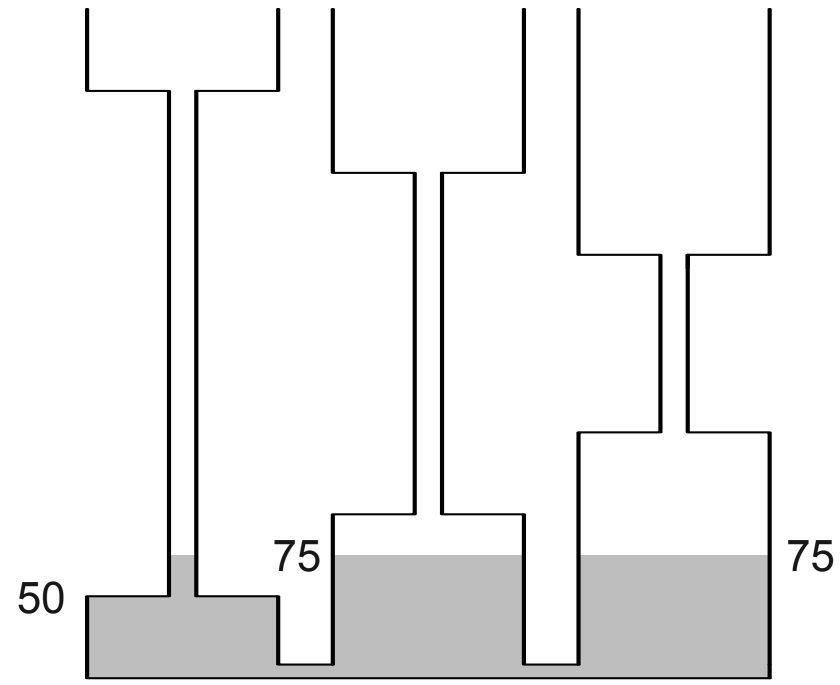
\includegraphics[scale=0.3]{images/CommunicatingVesselsExample.PNG}
    \caption{Solving a bankruptcy problem with communicating vessels ($E = 200$).}
\end{figure}

\subsection{Other Division Rules}
It is certainly not true that all division rules are consistent with the 2-person solutions, but quite a few are.
Take for example the \textbf{proportional rule}, where the estate is shared in proportion to the claims.
Similarly, the \textbf{constrained equal award rule (CEA)} states that the estate is shared equally among the claimants, but no claimant can receive more than their claim.
So if we have a bankruptcy problem $(E \text{ } | \text{ } c_1, c_2, ... , c_n)$, then the CEA-rule would try to give each of the $n$ claimants $\frac{E}{n}$.
However, if $c_1 < \frac{E}{n}$, then claimant $C_1$ just gets $c_1$ and the remainder $E - c_1$ should be divided among $C_2, C_3, ... , C_n$.
The CEA rule can be viewed as dividing the money one by one equally among the claimants who still have an outstanding claim.
It seems to be a natural procedure and there is proof that this rule has actually been used in law around 1200 AD.

\noindent
\\
Although the CEA solution is clearly different from the CG-consistent coalition solution, it has been shown that the coalition procedure assigns, for any bankruptcy problem $(E \text{ } | \text{ } c_1, c_2, ... , c_n)$ with $E < (c_1 + c_2 + ... + c_n)/2$, the same solution as the CEA rule would assign to the related bankruptcy problem where all claimants are claiming half as much: $(E \text{ } | \text{ } \frac{1}{2}c_1, \frac{1}{2}c_2, ... , \frac{1}{2}c_n)$.

\noindent
\\
Instead of sharing awards equally, one could also share losses equally.
Where for the CEA rule we make the exception that no claimant should get more than their claim, we should now share losses equally unless a claimant would get less than 0.
In this case the respective claimant would get 0 and the others continue sharing losses.
This is called the \textbf{constrained equal loss rule (CEL)}, and is the dual to the CEA rule.

%
% Topic 2 - Cooperative Games
%
\newpage
\section{Cooperative Games}
We started off our discussion on the Talmud table by explaining that the numbers in the table correspond exactly to the nucleolus of cooperative games.
In this section we will clarify these expressions, among some other issues.

\noindent
\\
An $n$-person \textbf{cooperative game} is given by a set of players $N = \{1, 2, ... , n\}$ and a function $v$ that assigns every subset $S$ of $N$ a non-negative real number $v(S)$.
Subsets of $N$ are called \textbf{coalitions}, with the set $N$ itself being called the \textbf{grand coalition}.
The function $v$ is known as the \textbf{characteristic function}.
An interpretation of this is that $v(S)$ expresses the \textit{value} of coalition $S$ (i.e. how much $S$ can achieve on its own).
A basic assumption is that the value of the empty set is always zero.

\noindent
\\
The idea of a cooperative game is that the $n$ players have to share the worth of the grand coalition $v(N)$.
Generally, in determining who is going to get what, the worth of the individual player in all coalitions plays a major role.

\noindent
\\
As an example, take a look at this 3-person cooperative game $(N, v)$:

\begin{table}[h]
    \centering
    \begin{tabular}{|c|cccccccc|}
    \hline
    $S$ & $\emptyset$ & 1 & 2 & 3 & 1,2 & 1,3 & 2,3 & 1,2,3 \\ \hline
    $v(S)$ & 0 & 1 & 3 & 4 & 4 & 5 & 8 & 10 \\ \hline
    \end{tabular}
\end{table}

\noindent
Where we have a set of players $N = \{1, 2, 3\}$, and the table above shows the worth of all coalitions.
The question is how these players 1, 2 and 3 should share 10, the worth of the grand coalition.

\noindent
\\
We leave this question for now to return to the Talmud table.
The Talmud table actually summarizes solutions for three different games: one in which the widows have to share 100, one where they have to share 200 and one where they have to share 300, while in each of the games their individual claims are 100, 200 and 300 respectively.
For each of these bankruptcy problems we can identify a cooperative game by defining the worth of a coalition $S$ to be the amount that remains if the widow(s) not in $S$ receive their claim first.
Let's examine these problems one by one:

\noindent
\\
The first column of the Talmud table gives the solution of the bankruptcy problem (100 $|$ 100, 200, 300).
Because each widow is claiming at least 100, the players outside $S$ are leaving nothing for the players in $S$, except when $S$ is the grand coalition.
This gives us the following cooperative game $(N, v_1)$:

\begin{table}[h]
    \centering
    \begin{tabular}{|c|cccccccc|}
    \hline
    $S$ & $\emptyset$ & 1 & 2 & 3 & 1,2 & 1,3 & 2,3 & 1,2,3 \\ \hline
    $v_1(S)$ & 0 & 0 & 0 & 0 & 0 & 0 & 0 & 100 \\ \hline
    \end{tabular}
\end{table}

\noindent
The second column of the Talmud table gives the solution of the bankruptcy problem (200 $|$ 100, 200, 300).
Since player 1 is claiming 100, player 2 and 3 are left with 100 when forming a coalition.
This means we get the following cooperative game $(N, v_2)$:

\begin{table}[h]
    \centering
    \begin{tabular}{|c|cccccccc|}
    \hline
    $S$ & $\emptyset$ & 1 & 2 & 3 & 1,2 & 1,3 & 2,3 & 1,2,3 \\ \hline
    $v_2(S)$ & 0 & 0 & 0 & 0 & 0 & 0 & 100 & 200 \\ \hline
    \end{tabular}
\end{table}

\newpage
\noindent
The third column of the Talmud table gives the solution of the bankruptcy problem (300 $|$ 100, 200, 300).
In similar fashion, we get the following cooperative game $(N, v_3)$:

\begin{table}[h]
    \centering
    \begin{tabular}{|c|cccccccc|}
    \hline
    $S$ & $\emptyset$ & 1 & 2 & 3 & 1,2 & 1,3 & 2,3 & 1,2,3 \\ \hline
    $v_3(S)$ & 0 & 0 & 0 & 0 & 0 & 100 & 200 & 300 \\ \hline
    \end{tabular}
\end{table}

\noindent
A solution to a cooperative game acts as a method to share the worth of the grand coalition among the individual players (this can be done in many ways, often upsetting at least one player).
One may see $v(N)$ as the result of cooperation among all players, while for each smaller coalition $S$ the amount $v(S)$ is what $S$ could have achieved on its own.
However, the $N$ individuals decided to cooperate and are now stuck having to share the joint profits or loses they made.

\subsection{The Core of a Cooperative Game}
We can denote an allocation of $v(N)$ to the players $1, 2, 3, ..., n$ by $(x_1, x_2, x_3, ..., x_n)$, where each player $i$ receives $x_i$ and $x_1 + x_2 + x_3 + ... + x_n = v(N)$.
Obviously each coalition $S$ would prefer to get a share of at least $v(S)$, but this may not be possible for all coalitions.
Allocations for which $x_i \geq v(i)$, for each player $i$, are called \textbf{individually rational}.
Allocations for which $x(S) = \sum_{i \in S} x_i \geq v(S)$, for each coalition $S$, are called \textbf{coalitionally rational}.
For any cooperative game $(N, v)$, the set of coalitionally rational allocations is called the \textbf{core}, and is denoted by $C(N, v)$.
The core of a game can be empty, one allocation, or a set of multiple allocations.

\noindent
\\
Let us return to the cooperative game $(N, v)$ given at the beginning of this chapter:

\begin{table}[h]
    \centering
    \begin{tabular}{|c|cccccccc|}
    \hline
    $S$ & $\emptyset$ & 1 & 2 & 3 & 1,2 & 1,3 & 2,3 & 1,2,3 \\ \hline
    $v(S)$ & 0 & 1 & 3 & 4 & 4 & 5 & 8 & 10 \\ \hline
    \end{tabular}
\end{table}

\noindent
An allocation $x = (x_1, x_2, x_3)$ for this 3-person game can be represented as a \textbf{vector} in $\mathbb{R}^3$, with

\[ x_1 + x_2 + x_3 = 10 \]

\noindent
We can visualize all possible allocations for this problem as a \textbf{plane} in $\mathbb{R}^3$:

\begin{figure}[h]
    \centering
    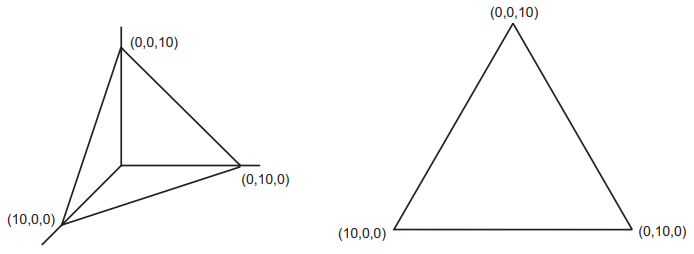
\includegraphics{images/plane.PNG}
\end{figure}

\newpage
\noindent
Given the table above, we can say that an allocation $x = (x_1, x_2, x_3)$ is individually rational if it satisfies:

\[ x_1 \geq 1 \]
\[ x_2 \geq 3 \]
\[ x_3 \geq 4 \]

\noindent
We can visualize these allocations by drawing lines in the plane above:

\begin{figure}[h]
    \centering
    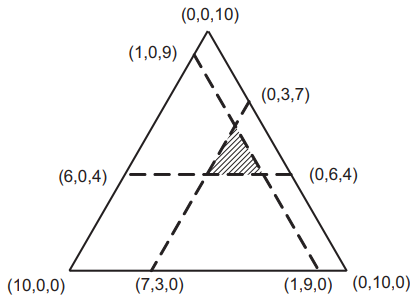
\includegraphics[scale=0.9]{images/planewithlines.PNG}
\end{figure}

\noindent
Here the shaded area corresponds to all possible individually rational allocations.
Similarly, we can say that an allocation $x = (x_1, x_2, x_3)$ is coalitionally rational if it also satisfies:
\vspace{-0.25cm}

\[ x_1 + x_2 \geq 4 \ \ (\text{or equivalently } x_3 \leq 6) \]
\[ x_1 + x_3 \geq 5 \ \ (\text{or equivalently } x_2 \leq 5) \]
\[ x_2 + x_3 \geq 8 \ \ (\text{or equivalently } x_1 \leq 2) \]

\noindent
We can once again visualize these allocations by drawing more lines:

\begin{figure}[h]
    \centering
    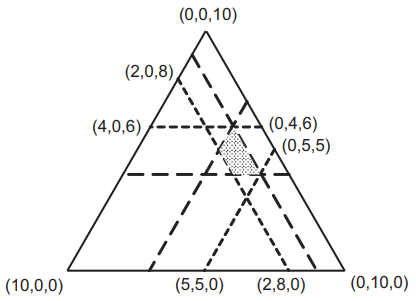
\includegraphics[scale=0.95]{images/planewithlines2.PNG}
\end{figure}

\noindent
From this we can conclude that the core of this game includes all allocations in the dotted area, with extreme points $(1, 3, 6)$, $(1, 5, 4)$, $(2, 4, 4)$ and $(2, 3, 5)$.

\newpage
\subsection{The Shapley Value}
Sometimes there are many allocations in the core of a game, while at other times there may be none at all.
In both cases it is unclear what allocations you should actually take.
To stop arguments on deciding which allocation should actually be taken, it is preferable to have a solution concept which always comes up with a unique allocation for any cooperative game.
The \textbf{Shapley value} is such a one-point solution concept.
In addition to this, the Shapley value is also closely related to several desirable properties for a solution: \textbf{anonymity}, \textbf{dummy} and \textbf{additivity}.

\noindent
\\
A solution concept has the property of \textbf{anonymity} if the actual solution does not depend on the names of the players.
For example, given our usual example game:

\begin{table}[h]
    \centering
    \begin{tabular}{|c|cccccccc|}
    \hline
    $S$ & $\emptyset$ & 1 & 2 & 3 & 1,2 & 1,3 & 2,3 & 1,2,3 \\ \hline
    $v(S)$ & 0 & 1 & 3 & 4 & 4 & 5 & 8 & 10 \\ \hline
    \end{tabular}
\end{table}

\noindent
We would like our solution to give players 1 and 2 the same amount as players 2 and 1 in the game where the roles are reversed:

\begin{table}[h]
    \centering
    \begin{tabular}{|c|cccccccc|}
    \hline
    $S$ & $\emptyset$ & 1 & 2 & 3 & 1,2 & 1,3 & 2,3 & 1,2,3 \\ \hline
    $v(S)$ & 0 & 3 & 1 & 4 & 4 & 8 & 5 & 10 \\ \hline
    \end{tabular}
\end{table}

\noindent
Player $i$ is called a \textbf{dummy player} if for any coalition $S$ not containing $i$ we have $v(S + i) = v(S) + v(i)$.
In other words, dummy player $i$ contributes the same amount $v(i)$ to any coalition.
For example:

\begin{table}[h]
    \centering
    \begin{tabular}{|c|cccccccc|}
    \hline
    $S$ & $\emptyset$ & 1 & 2 & 3 & 1,2 & 1,3 & 2,3 & 1,2,3 \\ \hline
    $v(S)$ & 0 & 1 & 3 & 4 & 6 & 5 & 7 & 10 \\ \hline
    \end{tabular}
\end{table}

\noindent
In the above game player 3 is a dummy player, because

\[ v(1, 3) = v(1) + v(3) \]
\[ v(2, 3) = v(2) + v(3) \]
\[ v(1, 2, 3) = v(1, 2) + v(3) \]

\noindent
Since dummy players do not really contribute to any profit or loss, it would be fair to give them $v(i)$ when it comes to dividing $v(N)$.
A solution concept that applies this rule is said to have the \textbf{dummy} property.

\noindent
\\
It would also be useful if several division problems among the same group of players could all be solved simultaneously.
If $(N, v)$ and $(N, w)$ are two cooperative games with the same set of players, then we define the cooperative game $(N, v + w)$ by taking $(v + w)(S) = v(S) + w(S)$ for all coalitions $S$.
For example, if we have the 3-person games $(N, v)$ and $(N, w)$ given by:

\newpage
\begin{table}[h]
    \centering
    \begin{tabular}{|c|cccccccc|}
    \hline
    $S$ & $\emptyset$ & 1 & 2 & 3 & 1,2 & 1,3 & 2,3 & 1,2,3 \\ \hline
    $v(S)$ & 0 & 3 & 1 & 4 & 4 & 8 & 5 & 10 \\ \hline
    \end{tabular}
\end{table}

\begin{table}[h]
    \centering
    \begin{tabular}{|c|cccccccc|}
    \hline
    $S$ & $\emptyset$ & 1 & 2 & 3 & 1,2 & 1,3 & 2,3 & 1,2,3 \\ \hline
    $w(S)$ & 0 & 1 & 3 & 4 & 6 & 5 & 7 & 10 \\ \hline
    \end{tabular}
\end{table}

\noindent
Then we would like to solve these games simultaneously by just looking at:

\begin{table}[h]
    \centering
    \begin{tabular}{|c|cccccccc|}
    \hline
    $S$ & $\emptyset$ & 1 & 2 & 3 & 1,2 & 1,3 & 2,3 & 1,2,3 \\ \hline
    $(v + w)(S)$ & 0 & 4 & 4 & 8 & 10 & 13 & 12 & 20 \\ \hline
    \end{tabular}
\end{table}

\noindent
A solution concept has the \textbf{additivity} property if for any two games $(N, v)$ and $(N, w)$ the solution of $(N, v + w)$ is the sum of the solutions of $(N, v)$ and $(N, w)$.

\noindent
\\
The \textbf{Shapley value} is a one-point solution concept induced by the anonymity, dummy and additivity properties, and is denoted by $\phi(N, v)$ or simply $\phi = (\phi_1, \phi_2, ... , \phi_n)$.
Every cooperative game has a Shapley value, but because of empty cores, this solution is not necessarily individually or coalitionally rational.

\noindent
\\
The Shapley value gives each player $i$ the average of their \textbf{marginal contributions}.
Assume that first player 1 enters a room and receives $v(1)$, then player 2 arrives and receives their marginal contribution $v(1, 2) - v(1)$, then player 3 arrives and receives $v(1, 2, 3) - v(1, 2)$, etc.
If we repeat this calculation for every possible order in which the players enter the room and then take the average, we get the Shapley value.
The Shapley value for player $i$ is given by:

\[ \phi_i(N, v) = \sum_{S \subset N \backslash \{i\}} \frac{s!(n - s - 1)!}{n!} (v(S + i) - v(S)) \]

\noindent
Where $s$ is the number of players in $S$.
This interpretation also provides a simple step-by-step method to calculate the Shapley value.
Given the following 3-person game:

\begin{table}[h!]
    \centering
    \begin{tabular}{|c|cccccccc|}
    \hline
    $S$ & $\emptyset$ & 1 & 2 & 3 & 1,2 & 1,3 & 2,3 & 1,2,3 \\ \hline
    $v(S)$ & 0 & 1 & 3 & 4 & 4 & 5 & 8 & 10 \\ \hline
    \end{tabular}
\end{table}

\noindent
We can calculate the Shapley value by calculating each player's marginal contribution for every possible order, which gives us $\phi = (\frac{8}{6}, \frac{23}{6}, \frac{29}{6})$:

\begin{table}[h!]
    \centering
    \begin{tabular}{c|ccc|}
    \cline{2-4}
     & 1 & 2 & 3 \\ \hline
    \multicolumn{1}{|c|}{1 - 2 - 3} & 1 & 3 & 6 \\
    \multicolumn{1}{|c|}{1 - 3 - 2} & 1 & 5 & 4 \\
    \multicolumn{1}{|c|}{2 - 1 - 3} & 1 & 3 & 6 \\
    \multicolumn{1}{|c|}{2 - 3 - 1} & 2 & 3 & 5 \\
    \multicolumn{1}{|c|}{3 - 1 - 2} & 1 & 5 & 4 \\
    \multicolumn{1}{|c|}{3 - 2 - 1} & 2 & 4 & 4 \\ \hline
    \multicolumn{1}{|c|}{column sums} & 8 & 23 & 29 \\
    \multicolumn{1}{|c|}{$\phi$} & $\frac{8}{6}$ & $\frac{23}{6}$ & $\frac{29}{6}$ \\ \hline
    \end{tabular}
\end{table}

\newpage
\subsection{The Nucleolus of a Cooperative Game}
The \textbf{nucleolus} is another one-point solution that can be found for any cooperative game.
Finding the nucleolus can be done using the following procedure:

\noindent
\\
If the core is \textbf{non-empty}, we simultaneously \textbf{increase} the worth of all coalitions, except the empty coalition $\emptyset$ and the grand coalition $N$, by the same amount.
This causes the "new core" to become smaller.
We continue increasing the worth of all coalitions until a further increment would give us an empty new core.
If that moment a single point remains, then we are done, it is the nucleolus.
Otherwise, there are two or more coalitions for which we cannot increase the coalitional worth any further without creating an empty core.
Therefore, we stop increasing the worth of these conflicting coalitions, but we keep increasing the worth of the other coalitions.
We proceed this way until we finally have a core consisting of just one point.
This point is the nucleolus of the game.

\noindent
\\
If the core is \textbf{empty}, we simultaneously \textbf{decrease} the worth of all coalitions (except the empty and grand coalition), until we arrive at a game with a non-empty core.
If we did not find a single-point core, we can proceed as before until we find the nucleolus.
Note that when starting from an empty core, we know right from the start that it is impossible to find a coalitionally rational solution.
The nucleolus may also not even be individually rational, since the procedure starts by decreasing the worth of all coalitions, including the 1-player coalitions.

\noindent
\\
Let us visualize this procedure through the usual example:

\begin{table}[h]
    \centering
    \begin{tabular}{|c|cccccccc|}
    \hline
    $S$ & $\emptyset$ & 1 & 2 & 3 & 1,2 & 1,3 & 2,3 & 1,2,3 \\ \hline
    $v(S)$ & 0 & 1 & 3 & 4 & 4 & 5 & 8 & 10 \\ \hline
    \end{tabular}
\end{table}

\noindent
We already saw earlier that the core of this game is non-empty.
The inequalities determining this core are:

\[ x_1 \geq 1 \text{ and } x_1 \leq 2 \]
\[ x_2 \geq 3 \text{ and } x_2 \leq 5 \]
\[ x_3 \geq 4 \text{ and } x_3 \leq 6 \]

\noindent
Notice that player 1 has the most narrow band of possibilities, since they should get something between 1 and 2.
If we increase the worth of all coalitions by 0.5, we get

\begin{table}[h]
    \centering
    \begin{tabular}{|c|cccccccc|}
    \hline
    $S$ & $\emptyset$ & 1 & 2 & 3 & 1,2 & 1,3 & 2,3 & 1,2,3 \\ \hline
    $v(S)$ & 0 & 1.5 & 3.5 & 4.5 & 4.5 & 5.5 & 8.5 & 10 \\ \hline
    \end{tabular}
\end{table}

\noindent
With core inequalities:

\[ x_1 \geq 1.5 \text{ and } x_1 \leq 1.5 \]
\[ x_2 \geq 3.5 \text{ and } x_2 \leq 4.5 \]
\[ x_3 \geq 4.5 \text{ and } x_3 \leq 5.5 \]

\newpage
\noindent
As $x_1$ is now fixed to 1.5, The new core will be a line segment in the $x_2x_3$-plane:

\begin{figure}[h]
    \centering
    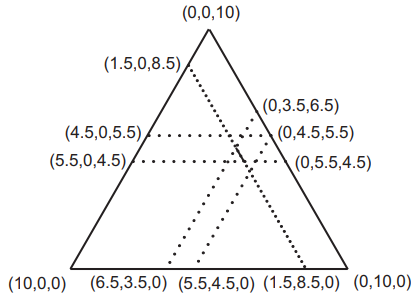
\includegraphics[scale=0.95]{images/planewithlines3.PNG}
\end{figure}

\noindent
Because we now have that $v(1) + v(2, 3) = 1.5 + 8.5 = 10$, any further increase in the worth of the coalitions $\{1\}$ and $\{2, 3\}$ would result in an empty core.
However, we can continue increasing the worth of coalitions $\{2\}$, $\{3\}$, $\{1, 2\}$ and $\{1, 3\}$.
This can be done by 0.25 at most:

\begin{table}[h]
    \centering
    \begin{tabular}{|c|cccccccc|}
    \hline
    $S$ & $\emptyset$ & 1 & 2 & 3 & 1,2 & 1,3 & 2,3 & 1,2,3 \\ \hline
    $v(S)$ & 0 & 1.5 & 3.75 & 4.75 & 4.75 & 5.75 & 8.5 & 10 \\ \hline
    \end{tabular}
\end{table}

\noindent
The core of this final adapted game is just one point: $(1.5, 3.75, 4.75)$.

\subsection{Minimizing Excess}
If for a game $(N, v)$ an allocation $(x_1, x_2, ... , x_n)$ is being considered as a solution, then one might wish to measure the level of satisfaction for each possible coalition with this solution.
A possible measure for this could be, for each coalition $S$, the difference between $v(S)$ and $x(S)$.
This difference is called the \textbf{excess} of coalition $S$ at $x$, and denoted by $e(S, x)$:

\[ e(S, x) = v(S) - x(S) \]

\noindent
Clearly, each coalition $S$ would prefer a solution $x$ for which $e(S, x)$ is as small as possible.
Therefore, as a "best" solution one might wish to take an $x$ for which the maximum excess over all coalitions is minimal.
If there are several solutions for which the maximum excess is the same, then one should take among these solutions the one with minimal second-highest excess.
Continuing this way, you eventually arrive at a unique solution, the \textbf{nucleolus}.

%
% Topic 3 - Rationality and Common Knowledge
%
\newpage
\section{Rationality and Common Knowledge}
Most game theoretic models involve an assumption that players are aware of the \textbf{game parameters} (e.g. the set of players, the set of actions, the payoff functions, the information structures, the goals of the players, etc.).
Not only does this mean that each player knows the game parameters, but also that each player knows that the other players know the game parameters, and that each player knows that the other players know that they know the game parameters, etc.

\noindent
\\
As for the goals of the players, the usual assumption is that the players choose their actions \textbf{rationally}.
This means that each player is assumed to choose their actions as to maximize their individual payoff, while totally neglecting the effect of these choices on the payoffs of the other players.
If a player has a possibility to improve their payoff, then they will always do so.

\noindent
\\
To get some idea of where these common knowledge and rationality assumptions may lead to, we examine a few exercises:

\subsection{Four Captured Dwarfs}
\textbf{Problem 1:}
Four dwarfs, A, B, C and D, have been captured by a witch.
In order to escape, the dwarfs must solve a difficult riddle with no discussion allowed.
The witch has put a hat on each dwarf's head.
Two hats are red and two hats are blue, but none of the dwarfs can see the color of their own hat.
The dwarfs also have limited visibility of each other: A can only see B and C, B can only see C, while C and D see nothing at all.
Each dwarf knows all the information mentioned above, and also knows that all the other dwarfs know this.
They are not allowed to communicate and the witch is watching.
If one of the dwarfs knows what color their hat is, they may tell the witch.
If the answer is correct and can be logically explained, then all dwarfs will be set free.
If the answer is wrong, then all dwarfs will be turned to frogs immediately.
How can the dwarfs escape?

\noindent
\\
\textbf{Solution:}
If dwarf A sees that both B and C are wearing the same color hat, then A knows that their own hat must be the opposite.
If dwarf A sees that B and C are wearing different color hats, then A does not know what color their hat is.
Dwarf B knows that A will know their hat color if B and C are wearing the same color hat.
This means that if A does not answer, then B knows that their hat is a different color than C's.

\subsection{More Dwarfs, More Hats}
\textbf{Problem 2:}
A group of 50 dwarfs is sitting in a circle, each wearing a red or a blue hat.
Each dwarf can see the color of the hat of all the other dwarfs, but not their own.
They know there is at least 1 red hat and at least 1 blue hat.
The King of the dwarfs will slowly count $1, 2, 3, 4, 5, ...$, and it is agreed by all that at each of these counts every dwarf will either stand up if they know their hat color, or remain seated.
What will happen when the King starts counting?

\noindent
\\
\textbf{Solution:}
If there is only 1 red hat, then the dwarf wearing the red hat will stand up at the first count.
If there are 2 red hats, then each dwarf wearing a red hat will only see 1 dwarf wearing a red hat.
If a dwarf wearing a red hat sees that the only dwarf wearing a red hat is not standing up at the first count, then they will know that the dwarf wearing a red hat must also be seeing a dwarf wearing a red hat.
Realizing this, both dwarfs will stand up at the second count.
This logic can be extended to any distribution of red and blue hats.

\newpage
\subsection{The Centipede Game}
\textbf{Problem 3:}
Two people, player 1 and 2, are involved in a decision problem.
Starting on the left, player 1 can choose between going down and ending the game, or going right and passing the decision to player 2.
As soon as one of the players decides to end the game, the players receive the amounts $a$ and $b$ as indicated in the following figure:

\begin{figure}[h]
    \centering
    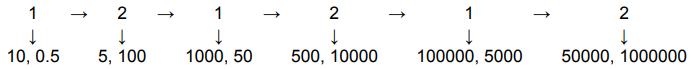
\includegraphics{images/centipedegame.PNG}
\end{figure}

\noindent
What will happen?

\noindent
\\
\textbf{Solution:}
If the game reaches the last node, then player 1 will always receive 50000.
This is less than the 100000 they would receive if they ended the game at the previous node.
Therefore, player 1 will always end the game at the second to last node.
Player 2, knowing this, will always end the game at the node before that, as they would receive 10000 instead of 5000.
Player 1 knows this as well, and will therefore always end the game at the node before that, etc.
Assuming both players play rationally, the game will always end at the first node, as there is no incentive for either player to go right.

\noindent
\\
This game is a special case of a \textbf{game in extensive form}.
These games can be visualized by means of a \textbf{decision tree}.
Play starts at a specific node, called the \textbf{root} of the tree.
Players then move in turns, making choices on which \textbf{branch} to follow at each node.
This continues until we reach one of the \textbf{leaves} of the tree, at which point each player gets their respective payoff.  

\noindent
\\
In the above example it is assumed that each player wants to maximize their individual payoff.
Each player wants to select the best \textbf{strategy} to play the game.
A strategy for a player is a complete plan of what to do in each of their decision nodes.

\begin{figure}[h]
    \centering
    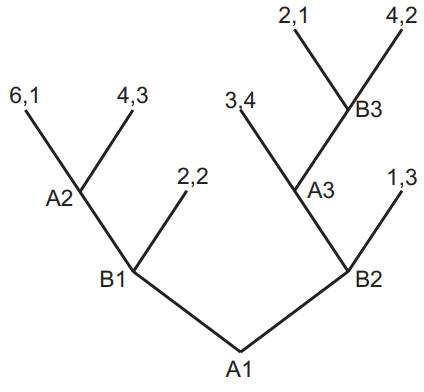
\includegraphics[scale=0.9]{images/gametree.PNG}
    \caption{An example of a game tree.}
\end{figure}

%
% Topic 4 - Games in Normal Form
%
\newpage
\section{Games in Normal Form}
A game in \textbf{normal form} is defined by a triple $\left\langle S, \left(A^k\right)_{k \in S}, \left(r^k\right)_{k \in S} \right\rangle$, where $S = \{ 0, 1, 2, ... , n \}$ is the set of players, $A^k$ is the set of strategies for player $k$ and $r^k : A^k \rightarrow \mathbb{R}$ is the payoff function for player $k$.
Using the \textbf{rationality} assumption we can assume that each player knows the set of players, all possible actions each player can choose and the possible payoffs for each combination of actions.
We also assume that each player wants to maximize their individual payoff, and knows their opponents want to maximize their individual payoff.
Lastly, all players are assumed to choose their actions simultaneously and independent of each other.

\noindent
\\
In this chapter we will illustrate these concepts by looking at 2-person normal form games, also called \textbf{bimatrix games}.
These games can be represented by a matrix with two numbers in each entry.
It is usual to have the rows correspond to the strategies of player 1, while the columns correspond to the strategies of player 2 (in the context of bimatrix games, strategies are often called \textbf{actions}).
A bimatrix game in which players 1 and 2 respectively have $m$ and $n$ actions can be represented by a matrix of the form:

\[ (A, B) = [a_{ij}, b_{ij}] = \begin{pmatrix}
    a_{11}, b_{11} & a_{12}, b_{12} & \dots & a_{1j}, b_{1j} & \dots & a_{1n}, b_{1n} \\
    a_{21}, b_{21} & a_{22}, b_{22} & \dots & a_{2j}, b_{2j} & \dots & a_{2n}, b_{2n} \\
    \vdots & \vdots & & \vdots & & \vdots \\
    a_{i1}, b_{i1} & a_{i2}, b_{i2} & \dots & a_{ij}, b_{ij} & \dots & a_{in}, b_{in} \\
    \vdots & \vdots & & \vdots & & \vdots \\
    a_{m1}, b_{m1} & a_{m2}, b_{m2} & \dots & a_{mj}, b_{mj} & \dots & a_{mn}, b_{mn}
\end{pmatrix} \]

\subsection{Nash-Equilibrium}
Player 1 would like to choose row $i$ to maximize their payoff $a_{i\dots}$, while player 2 would like to choose column $j$ to maximize their payoff $b_{\dots j}$.
Their final payoff will of course also be dependent on the choice of the other player.
This means both players are looking for the \textbf{best replies} to the other player's choice.
Player 1 would like to have chosen some $i^*$ in such a way that, against $j^*$ chosen by player 2, they could not have done any better:

\[ a_{i^* j^*} = \max_i a_{ij^*} \]

\noindent
Clearly, player 2 would also want their action $j^*$ to be the best reply to $i^*$:

\[ b_{i^* j^*} = \max_j a_{i^*j} \]

\noindent
A pair of actions / strategies that are best replies against each other is called a \textbf{Nash-equilibrium}.
Take a look at the following bimatrix game:

\[ \begin{pmatrix}
    2,1 & 0,0 \\
    0,0 & 1,2
\end{pmatrix} \]

\noindent
This game has two equilibria: $(1, 1)$ and $(2, 2)$.
Note that the payoffs of these equilibria are not the same; player 1 would prefer to play $(1, 1)$, but player 2 would prefer to play $(2, 2)$.
This shows that the payoffs of a Nash-equilibrium are not necessarily optimal for both players.

\newpage
\noindent
What happens if we change the payoffs slightly?

\[ \begin{pmatrix}
    2,0 & 0,2 \\
    0,1 & 1,0
\end{pmatrix} \]

\noindent
We can quickly observe that there is no pair of actions $(i^*, j^*)$ that are best replies to each other in this game.
Let's imagine that in this example player 2 has somehow found out what player 1 is going to do, then, clearly, player 1 will end up only getting 0.
Player 1 could of course anticipate player 2's behavior, but then we would quickly find ourselves in an infinite loop.

\noindent
\\
A better way for player 1 to camouflage their intention would be to choose their action randomly (e.g. flipping a coin to decide if they are going to pick 1 or 2).
If player 2 finds out about this plan, they need to evaluate what is best for them:

\begin{enumerate}
    \item If player 2 chooses left, then with probability $\frac{1}{2}$ they will receive 0 and with probability $\frac{1}{2}$ they will receive 1.
    This means player 2's \textbf{expected payoff} for choosing left is $\frac{1}{2} \cdot 0 + \frac{1}{2} \cdot 1 = \frac{1}{2}$.
    \item If player 2 chooses right, then with probability $\frac{1}{2}$ they will receive 2 and with probability $\frac{1}{2}$ they will receive 0.
    This means player 2's \textbf{expected payoff} for choosing right is $\frac{1}{2} \cdot 2 + \frac{1}{2} \cdot 0 = 1$.
\end{enumerate}

\noindent
Assuming player 1 decides their choice using a coin flip, it seems better for player 2 to choose right.
Using probability devices, player 1 could choose action 1 with any probability they like.
This drastically increases player 1's set of possible actions.
We call these probabilistic actions \textbf{mixed actions}.
For player 1, a mixed action in an $m \times n$-bimatrix game is a vector $(p_1, p_2, ... , p_m)$, where $p_i \geq 0$ is the probability of choosing action $i$, and $p_1 + p_2 + ... + p_m = 1$.

\subsection{Best Reply Functions}
For 2-person games, a structural approach to find strategies that are best replies to each other is by drawing a diagram of the \textbf{best reply functions}:

\[ B_1(q) = \{ x \in (0, 1) : (1 - x, x) \text{ is a best reply for player 1 against } (1 - q, q) \} \]
\[ B_2(p) = \{ y \in (0, 1) : (1 - y, y) \text{ is a best reply for player 2 against } (1 - p, p) \} \]

\noindent
With $p, q \in (0, 1)$ for player 2 and 1 respectively.

\begin{figure}[h!]
    \centering
    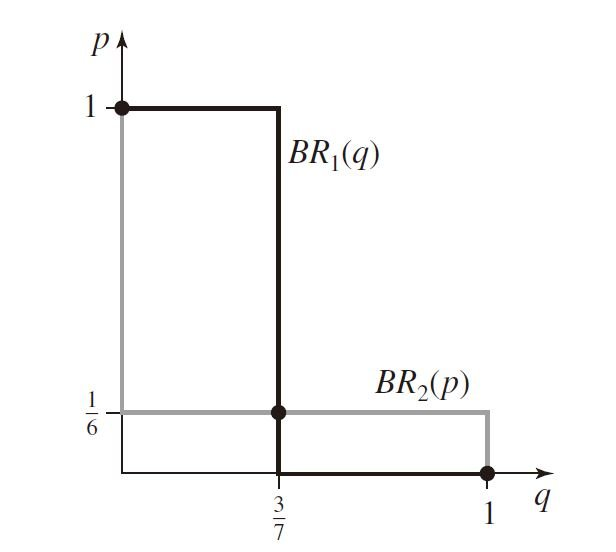
\includegraphics[scale=0.5]{images/bestreplydiagram.png}
    \caption{An example of a \textbf{best reply diagram} with 3 equilibria.}
\end{figure}

\newpage
\noindent
It has been shown that any $n$-player game, in which each player has finitely many actions, has at least one Nash-equilibrium in mixed actions.
If there is more than one, it is important to realize that the payoffs of these equilibria may be very much different from each other.
For example, if the players in the bimatrix game mentioned at the start of this chapter want to play the mixed equilibrium:

\[ \left( \left( \frac{2}{3},\frac{1}{3} \right) , \left( \frac{1}{3},\frac{2}{3} \right) \right) \]

\noindent
Then with probability $\frac{2}{9}$ this would lead to the players ending up in the situation $(1, 1)$ with payoffs $2, 1$; with probability $\frac{2}{9}$ it would yield the situation $(2, 2)$ with payoffs $1, 2$; but also, with probability $\frac{5}{9}$ play would end in one of the entries with payoffs $0, 0$.
The expected payoff for the players would be:

\[ \frac{2}{9} \cdot (2, 1) + \frac{2}{9} \cdot (1, 2) + \frac{5}{9} \cdot (0, 0) = \left( \frac{6}{9},\frac{6}{9} \right) \]

\noindent
In expected payoff it is important to realize that, assuming the players are independently trying to maximize their individual payoff, receiving a payoff of $1.000.000$ with probability $\frac{1}{2}$ or losing $1.000.000$ with probability $\frac{1}{2}$ is worth just as much as receiving a payoff of 0.
Of course, in real life not everyone would like to take the risk of having to pay $1.000.000$, but for this course we assume that the players are \textbf{risk neutral}.

\subsection{Correlated Equilibrium}
Of course, in the above example, we would prefer a solution that never yields a $(0, 0)$-payoff.
A solution that would yield a payoff like $\left( 1\frac{1}{2}, 1\frac{1}{2} \right)$ would seem to be a fair solution, but we cannot reach this solution if we do not allow players to \textbf{correlate} their actions by choosing $(1, 1)$ with probability $\frac{1}{2}$ and $(2, 2)$ with probability $\frac{1}{2}$.
If player 1 plays $(1 - p, p)$ and player 2 plays $(1 - q, q)$ then, no matter how we choose $p$ and $q$, we can never create an outcome that yields $(1, 1)$ with probability $\frac{1}{2}$ and $(2, 2)$ with probability $\frac{1}{2}$.
The only way to achieve this is by having both players obey the outcome of a single probability experiment.
Such a probability experiment is called a \textbf{correlation device}.
For a 2-person game, it is a matrix

\[ P = \begin{pmatrix}
    p_{11} & p_{12} \\
    p_{21} & p_{22}
\end{pmatrix} \]

\noindent
with $p_{ij} \geq 0$ for all $i$ and $j$, and $p_{11} + p_{12} + p_{21} + p_{22} = 1$.

\noindent
\\
The idea of correlating the actions of players lead to the concept of a \textbf{correlated equilibrium}.
A correlated equilibrium is a specific correlation device $P^*$ which has certain stability properties.
The idea of this concept is that some arbitrator will select one of the entries of the matrix according to the correlation device $P^*$.
The matrix $P^*$ is known to the player, but as far as the outcome of the chance experiment is concerned, each player shall only be told their own action.
Note that, no matter the outcome of the probability experiment, the arbitrator's advice for each player should be a best reply to what the arbitrator expects the other player to do.
Take the following example:

\newpage
\noindent
Given the following correlated equilibrium:

\[ P = \begin{pmatrix}
    0.5 & 0.2 \\
    0 & 0.3
\end{pmatrix} \]

\noindent
Suppose that, unknown to the players, the arbitrator selected entry $(1, 1)$.
The arbitrator will advise player 1 to play 1, and player 2 to play 1.
If player 1 is told to play 1, then, knowing $P^*$, player 1 knows that with probability $\frac{0.5}{0.5 + 0.2} = \frac{5}{7}$ player 2 has been told to play 1 as well.
Player 1 expects player 2 to play according to the mixed strategy $(\frac{5}{7}, \frac{2}{7})$.
Against this mixed action a best reply for player 1 is to play 1.
Likewise, if player 2 is told to play 1, then they expect player 1 to play 1, for which 1 is a best reply for player 2.

\noindent
\\
Suppose that, unknown to the players, the arbitrator selected entry $(2, 2)$.
The arbitrator will advise player 1 to play 2, and player 2 to play 2.
If player 1 is told to play 2, then, knowing $P^*$, player 1 knows for sure that player 2 has been told to play 2 as well, for which 2 is a best reply for player 1.
Likewise, if player 2 is told to play 2, then they expect player 1 to play according to the mixed strategy $(\frac{2}{5}, \frac{3}{5})$, for which 2 is a best reply for player 2.

\noindent
\\
Suppose that, unknown to the players, the arbitrator selected entry $(1, 2)$.
The arbitrator will advise player 1 to play 1, and player 2 to play 2.
If player 1 is told to play 1, then, knowing $P^*$, player 1 expects player 2 to play according to the mixed strategy $(\frac{5}{7}, \frac{2}{7})$, for which 1 is a best reply for player 1.
If player 2 is told to play 2, then they expect player 1 to play according to the mixed action $(\frac{2}{5}, \frac{3}{5})$, for which 2 is a best reply for player 2.

\noindent
\\
Since for every outcome of the probability experiment it is best for each player to follow the arbitrator's advise, the distribution $P$ is called a correlated equilibrium.
When playing this correlated equilibrium, the expected payoffs for the players are:

\[ 0.5 \cdot (2, 1) + 0.2 \cdot (0, 0) + 0.3 \cdot (1, 2) = (1.3, 1.1) \]

\subsection{Dominated Strategies}
A famous bimatrix game is the \textbf{Prisoner's Dilemma}:

\[ \begin{pmatrix}
    3,3 & 0,5 \\
    5,0 & 1,1
\end{pmatrix} \]

\noindent
In this game, we can observe that for player 1 the second row is strictly better than the first row.
No matter what column we pick, the second row will always yield a higher payoff for player 1.
We say that the first row is \textbf{dominated} by the second row.
Similarly, we can say that the first column is dominated by the second column for player 2.

\noindent
\\
Clearly, in any equilibrium none of the players is going to play (with positive probability) a dominated strategy.
This means that we can remove the dominated strategies from the game without changing the set of equilibria.

%
% Topic 5 - Matrix Games
%
\newpage
\section{Matrix Games}
In this section we will examine a special type of games in normal form: \textbf{matrix games}.
These are bimatrix games $(A, B)$ for which $B = -A$.
This means that for any choice $i$ of player 1 and $j$ for player 2, we have $b_{ij} = -a_{ij}$.
These games are often called \textbf{zero-sum games}, since the sum of the payoffs for the players is always 0.
For a matrix game we immediately know the payoffs to player 2 as soon as we know the payoffs to player 1.
Therefore, we can represent a matrix game by just giving the matrix $A$ of payoffs to player 1.
An important realization in matrix games is that the assumption that player 2 is trying to maximize their own payoff, is the same as the assumption that player 2 is trying to minimize player 1's payoff.

\subsection{Saddle Points}
Take the following matrix game:

\[ A = \begin{pmatrix}
    -3 & 5 \\
    0 & 1
\end{pmatrix} \]

\noindent
For player 2, the second column is being dominated by the first column.
This means that player 2 will never play the second column.
Player 1, knowing this, will always play the second row to maximize their payoff.
This means that the strategy $(2, 1)$ is a Nash-equilibrium.

\noindent
\\
If a matrix game has an equilibrium in pure actions $(i^*, j^*)$, then we call this equilibrium a \textbf{saddle point}.
This means that, by definition, the related payoff is the maximum of column $j^*$ and at the same time the minimum of row $i^*$:

\[ a_{i^* j} \geq a_{i^* j^*} \geq a_{i j^*} \]

\noindent
We could also write this expression as:

\[ \min_{j} a_{i^* j} = a_{i^* j^*} = \max_{i} a_{i j^*} \]

\noindent
Through some rewriting, we can find the following equivalent statement:

\[ \max_{i} \min_{j} a_{ij} = a_{i^* j^*} = \min_{j} \max_{i} a_{ij} \]

\noindent
This means that, if we have a saddle point, then its payoff equals the \textbf{largest row minimum}, and the \textbf{smallest column maximum}.
Conversely, if the largest row minimum equals the smallest column maximum, then there exists at least one saddle point.

\subsection{The Minimax-Theorem}
Take a look at the following matrix game:

\[ A = \begin{pmatrix}
    0 & -2 & 5 \\
    4 & 10 & -1
\end{pmatrix} \]

\noindent
We can find that the largest row minimum $\max_{i} \min_{j} a_{ij} = -1$ and the smallest column maximum $\min_{j} \max_{i} a_{ij} = 4$.
Therefore, by playing pure actions, player 1 can be sure of getting at least -1, while player 2 can be sure of paying at most 4.
However, these points are not equilibria, as the opposing player could play better moves in each situation.

\newpage
\noindent
Like in bimatrix games, the players might be able to guarantee a better payoff by playing mixed actions.

\noindent
\\
For player 1 a mixed action can be given as $(1 - p, p)$, where $p \in (0, 1)$ is the probability of playing the bottom row.
Let $f_j(p)$ denote the expected payoff for player 1 if they play $(1 - p, p)$, while player 2 plays column $j$.
We can visualize these functions in the following plot:

\begin{figure}[h]
    \centering
    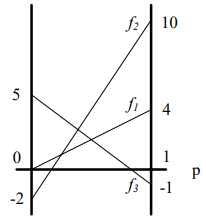
\includegraphics{images/f123plot.PNG}
\end{figure}

\noindent
Player 1 wants to maximize their minimum (expected) payoff, which can be visualized as the function $f_-(p) = \min \{ f_j(p) \}$:

\begin{figure}[h]
    \centering
    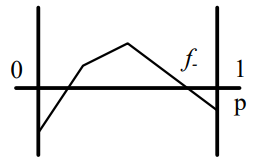
\includegraphics{images/fminus.PNG}
\end{figure}

\noindent
If player 1 wishes to maximize their minimum payoff, then they should choose $p$ such that $f_-(p)$ is maximized.
For this particular example, that $p$ can be computed by solving the equation:

\begin{table}[h]
    \centering
    \begin{tabular}{rcll}
    $f_1(p)$ & $=$ & $f_3(p)$ & or, written differently: \\
    $4p$ & $=$ & $-6p + 5$ & 
    \end{tabular}
\end{table}

\noindent
This gives $p = \frac{1}{2}$ and $f_1(p) = f_3(p) = 2$.
Thus, by playing the mixed action $(\frac{1}{2}, \frac{1}{2})$, player 1 knows that their expected payoff is going to be at least 2.

\noindent
\\
We now examine the situation from player 2's perspective.
If player 2 uses a mixed action $q = (q_1, q_2, q_3)$ and player 1 plays row 1, then player 1 gets the following expected payoff:
\[ E_1(q) = 0 \cdot q_1 - 2 \cdot q_2 + 5 \cdot q_3 \]

\noindent
If player 1 plays row 2, then player 1 gets the following expected payoff:
\[ E_2(q) = 4 \cdot q_1 + 10 \cdot q_2 - 1 \cdot q_3 \]

\noindent
If player 1 plays the mixed strategy $(1 - p, p)$, then player 1's expected payoff is:
\[ (1 - p) \cdot E_1(q) + p \cdot E_2(q) \]

\noindent
The maximum amount player 2 will have to pay, in expectation, is $\max \{ E_1(q), E_2(q) \}$.

\newpage
\noindent
Player 2 will try to choose their mixed action $q$ in such a way as to keep $\max \{ E_1(q), E_2(q) \}$ as small as possible.
We can visualize the payoff for player 2 as a weighted mixture of the separate columns $f_q(p) = q_1 \cdot f_1(p) + q_2 \cdot f_2(p) + q_3 \cdot f_3(p)$: 

\begin{figure}[h]
    \centering
    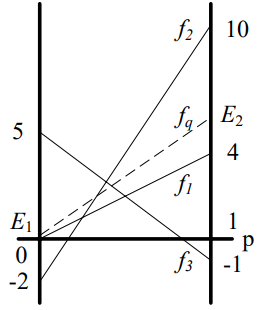
\includegraphics[scale=0.8]{images/fqplot.PNG}
\end{figure}

\noindent
What $q$ should player 2 choose?
We know that player 1 will choose $p = \frac{1}{2}$ because this means that player 1's expected payoff is at least $f_1(\frac{1}{2}) = f_3(\frac{1}{2}) = 2$.
We can also calculate that $f_2(\frac{1}{2}) = 4$.
This means that if player 2 would take $q_2 \neq 0$, then $f_q(\frac{1}{2}) > 2$.
The only way player 2 could be able to make sure that they should never pay more than 2 (in expectation) is by taking $q_2 = 0$, and by taking $q_1$ and $q_3$ such that $E_1(q) = E_2(q) = 2$:

\begin{figure}[h]
    \centering
    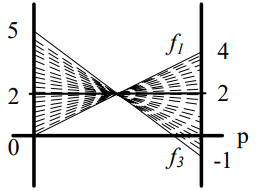
\includegraphics[scale=0.9]{images/f1f3fq.PNG}
\end{figure}

\noindent
To do so, player 2 should balance the graphs of $f_1$ and $f_3$.
To achieve this balance, we need to turn the picture and look at the length of the "arms":

\begin{figure}[h]
    \centering
    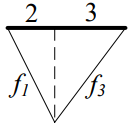
\includegraphics[scale=0.8]{images/f1f3arms.PNG}
\end{figure}

\noindent
This shows that $q_1$ should be $1\frac{1}{2}$ times as big as $q_3$.
Thus, by playing the mixed strategy $(\frac{3}{5}, 0, \frac{2}{5})$ player 2 can be sure that the expected payoff to player 1 is not going to be more than 2.

\noindent
\\
If for a matrix game $A$ there are mixed actions $p^* = (p^*_1, p^*_2, ... , p^*_m)$ for player 1 and $q^* = (q^*_1, q^*_2, ... , q^*_n)$ for player 2, and a number $v \in \mathbb{R}$ such that for all mixed actions $p$ and $q$ we have:

\[ p^*Aq \geq v \geq pAq^* \]

\noindent
Then $v$ is called the \textbf{value} of $A$ and mixed actions $p^*, q^*$ are called the \textbf{optimal mixed actions} for player 1 and player 2 respectively.
It has been proved under the \textbf{minimax-theorem} that every matrix game has a value, and that there are optimal mixed actions for both players.

\newpage
\subsection{Proof of the Minimax-Theorem}
To proof the minimax-theorem, we can use \textbf{linear programming}.
If player 1 wants to find an optimal strategy in a matrix game, then they are trying to find the highest value $v$ such that each column will get them an expected payoff of at least $v$.
Mathematically, this can be written as:
\begin{align*}
    &\mathrm{max} \quad v \\[2pt]
    &\mathrm{s.t.} \quad
    \begin{array}[t]{l c l}
    \sum_{i = 1}^m p_i a_{ij} & \geq & v \quad \mathrm{for} \quad j = 1, 2, ... , n\\
    \sum_{i = 1}^m p_i & = & 1
    \end{array}\\
    &\mathrm{and} \quad p_i \geq 0 \quad \mathrm{for} \quad i = 1, 2, ... , m
\end{align*}

\noindent
Similarly, player 2 can also find a solution for the matrix game by solving a similar linear programming problem:
\begin{align*}
    &\mathrm{min} \quad w \\[2pt]
    &\mathrm{s.t.} \quad
    \begin{array}[t]{l c l}
    \sum_{j = 1}^n a_{ij} q_j & \leq & w \quad \mathrm{for} \quad i = 1, 2, ... , m\\
    \sum_{j = 1}^n q_j & = & 1
    \end{array}\\
    &\mathrm{and} \quad q_j \geq 0 \quad \mathrm{for} \quad j = 1, 2, ... , n
\end{align*}
 
\noindent
If we assume that all entries of $A$ are positive, which can be done without loss of generality (raising all entries by a constant will raise the value of the game by the same constant), then we know for sure that both $v$ and $w$ are positive.
We can therefore rewrite the first problem as:
\begin{align*}
    &\mathrm{min} \quad \begin{array}[t]{l c l}
    \frac{1}{v} & = & \sum_{i = 1}^m x_i
    \end{array}\\[2pt]
    &\mathrm{s.t.} \quad
    \begin{array}[t]{l c l}
    \sum_{i = 1}^m x_i a_{ij} & \geq & 1 \quad \mathrm{for} \quad j = 1, 2, ... , n
    \end{array}\\
    &\mathrm{and} \quad x_i \geq 0 \quad \mathrm{for} \quad i = 1, 2, ... , m
\end{align*}

\noindent
Where $x_i = \frac{p_i}{v}$.
Similarly, using $y_j = \frac{q_j}{w}$, the linear program for player 2 can be rewritten as:
\begin{align*}
    &\mathrm{max} \quad \begin{array}[t]{l c l}
    \frac{1}{w} & = & \sum_{j = 1}^n y_j
    \end{array}\\[2pt]
    &\mathrm{s.t.} \quad
    \begin{array}[t]{l c l}
    \sum_{j = 1}^n a_{ij} y_j & \leq & 1 \quad \mathrm{for} \quad i = 1, 2, ... , m
    \end{array}\\
    &\mathrm{and} \quad y_j \geq 0 \quad \mathrm{for} \quad j = 1, 2, ... , n
\end{align*}

\noindent
Notice how these reformulated linear programs are each other's duals.
By the strong duality theorem, we know that the optimal values $\frac{1}{v^*}$ and $\frac{1}{w^*}$ of these problems are equal.
As such, this provides a proof for the minimax-theorem.

\subsection{Fictitious Play}
So far we know how to solve a matrix game if we can reduce it to one with only two rows or columns by eliminating dominated actions, but what if we cannot reduce the game?
One option is to use the linear programs from the previous section, but this is not always optimal.
Another option is to use \textbf{fictitious play}.
Fictitious play is an iterative procedure that can be interpreted as having the players play the game infinitely many times, where at each point in time (\textbf{stage}) each player is playing a best reply to the mixed action that fits best with the opponents observed behavior.

\newpage
\noindent
As an example:
If, in a 7x8 matrix game, upon arrival at stage 11 player 1 observes that player 2 has played the actions 1, 3, 4 and 6 respectively 2, 1, 4 and 3 times, then player 1 will choose a row that is a best reply against the mixed action $(\frac{2}{10}, 0, \frac{1}{10}, \frac{4}{10}, 0, \frac{3}{10}, 0, 0)$.
Similarly, player 2, having observed player 1 choosing the actions 3, 5 and 6 respectively 4, 5 and 1 times, will choose a column that is a best reply against the mixed action $(0, 0, \frac{4}{10}, 0, \frac{5}{10}, \frac{1}{10}, 0)$.

\noindent
\\
The fictitious play process can start with any two arbitrary actions.
The mixed actions that result from the players' observations will converge to the optimal mixed actions, while the related payoff will converge to the value of the matrix game.
If at a certain stage there is more than one pure best reply to the observed mixed action of the opponent, then we always take the smallest action as a tiebreaker rule (i.e. if both action 3 and 5 are best replies, then we choose action 3).
Note that this method only works for zero-sum games.

%
% Topic 6 - Calculating Equilibria in Bimatrix Games
%
\newpage
\section{Calculating Equilibria in Bimatrix Games}
Let $(A, B)$ be a bimatrix game in which player 1 has $m$ actions and player 2 has $n$ actions, i.e. there are $m$ rows and $n$ columns.
As before, player 1 can play a mixed action $p = (p_1, p_2, ... , p_m)$ and player 2 can play a mixed action $q = (q_1, q_2, ... , q_n)$.
We will denote the set of mixed actions of player 1 by $P$ and the set of mixed actions of player 2 by $Q$.
However, we will make one notational adjustment in order to have a unique name for each action:
Instead of listing the actions of player 2 as $1, 2, ... , n$, we will denote them as $m + 1, m + 2, ... , m + n$.
As such we will use the notation $p = (p_1, p_2, ... , p_m)$ for an element in $P$ and $q = (q_{m + 1}, q_{m + 2}, ... , q_{m + n})$ for an element in $Q$.

\subsection{Completely Labeled Actions}
An equilibrium is a pair of actions that are best replies to each other.
In a little more detail we can state:
A pair of actions $(p, q)$ is an equilibrium if and only if for each action $i$ for player 1 we have that $p_i > 0$ implies $i$ is a best reply to $q$, and for each action $j$ for player 2 we have that $q_j > 0$ implies $j$ is a best reply to $p$.
Let $u(q)$ be the best reply payoff for player 1 against $q$, i.e. $u(q)$ is the highest expected payoff player 1 can get against $q$.
Similarly, let $w(p)$ be the best reply payoff for player 2 against $p$.
We can write this as:

\[ u(q) = \max_i \sum_{j = m + 1}^{m + n} a_{ij} q_j \quad \text{and} \quad w(p) = \max_j \sum_{i = 1}^{m} p_i b_{ij} \]

\noindent
For every $i$ and $j$ we can define non-negative \textbf{slack variables}:

\[ r_i(q) = u(q) - \sum_{j = m + 1}^{m + n} a_{ij} q_j \quad \text{and} \quad s_j(p) = w(p) - \sum_{i = 1}^{m} p_i b_{ij} \]

\noindent
Note that $i$ is a best reply for player 1 against $q$ if and only if $r_i(q) = 0$, and $j$ is a best reply for player 2 against $p$ if and only if $s_j(p) = 0$.
For each $p \in P$ and $q \in Q$ we can define the following \textbf{labels}:

\begin{table}[h]
    \centering
    \begin{tabular}{ccccc}
    $L^1(p)$ & $=$ & $\{ i : p_i = 0 \}$ & $\cup$ & $\{ j : s_j(p) = 0 \}$ \\
    $L^2(q)$ & $=$ & $\{ i : r_i(q) = 0 \}$ & $\cup$ & $\{ j : q_j = 0 \}$ \\
    $L(p, q)$ & $=$ & $L^1(p)$ & $\cup$ & $L^2(q)$
    \end{tabular}
\end{table}

\noindent
A pair of actions $(p, q)$ is called \textbf{completely labeled} if $L(p, q) = \{ 1, 2, 3, ... , m + n \}$.
In view of the above definition, a pair of actions $(p, q)$ is an equilibrium if and only if for each action $i$ for player 1 we have that $i \in L(p, q)$, and at the same time for each action $j$ for player 2 we have that $j \in L(p, q)$.
In other words, a pair of actions $(p, q)$ is an equilibrium if and only if $L(p, q)$ is completely labeled.
A pair of actions is called \textbf{almost completely labeled} if there is only one element missing from this set.

\subsection{The Lemke-Howson Algorithm}
In view of the above observations, the problem of finding an equilibrium in a bimatrix game $(A, B)$ can be formulated as:

\newpage
\noindent
FIND $u$, $w$ and vectors:

\begin{table}[h]
    \centering
    \begin{tabular}{rcl}
    $p = (p_1, p_2, ... , p_m) \geq 0$ & \quad and \quad & $r = (r_1, r_2, ... , r_m) \geq 0$ \\
    $q = (q_{m + 1}, q_{m + 2}, ... , q_{m + n}) \geq 0$ & \quad and \quad & $s = (s_{m + 1}, s_{m + 2}, ... , s_{m + n}) \geq 0$
    \end{tabular}
\end{table}

\noindent
SUBJECT TO CONSTRAINTS:

\begin{table}[h]
    \centering
    \begin{tabular}{rcl}
        $\sum_i p_i = \sum_j q_j = 1$ & & \\
        $\sum_j a_{ij} q_j + r_i = u$ & \quad & for $i = 1, 2, ... , m$ \\
        $\sum_i p_i b_{ij} + s_j = w$ & \quad & for $j = m + 1, m + 2, ... , m + n$ \\
        $p_i r_i = 0$ & \quad & for $i = 1, 2, ... , m$ \\
        $q_j s_j = 0$ & \quad & for $j = m + 1, m + 2, ... , m + n$
    \end{tabular}
\end{table}

\noindent
The last $m + n$ constraints in this formulation guarantee that labels correspond to actions that are either best replies or have a weight of 0.
Note that these constraints are the only non-linear equations in this formulation.
Mathematicians Lemke and Howson discovered an approach similar to the Simplex method that can be used to solve this non-linear problem.
Just like the Simplex method moves from one corner point solution to another corner point solution until an optimal one is found, the \textbf{Lemke-Howson algorithm} moves along almost completely labeled pairs of actions until it finds a completely labeled pair of actions, which is an equilibrium.

\noindent
\\
While the Simplex method consists of performing pivoting steps in a tableau, the Lemke-Howson algorithm consists of performing pivoting steps in two tableaux.
These steps are taken in such a way that we are only changing the action of one player at a time, for alternating players.
Our path will move along almost completely labeled pairs of actions, which have the property that exactly one label appears twice.
We will continue removing the double label until we find the missing label.
An almost completely labeled pair of actions is called \textbf{ACL-$k$} if label $k$ is missing.
If we start our path with an ACL-$k$ pair of actions, then our path will only move along ACL-$k$ pairs until we find a completely labeled pair.
As such the path will be called a \textbf{$k$-path}.
Before turning to the pivotal approach, examine the following graphical example:

\subsection{Graphical Procedure}
We examine the game $(A, B)$ given by:

\[ A = \begin{pmatrix}
    12 & 2 & 2 \\
    10 & 8 & 3 \\
    9 & 4 & 6
\end{pmatrix} \quad \text{and} \quad
B = \begin{pmatrix}
    2 & 0 & 3 \\
    2 & 3 & 0 \\
    1 & 0 & 0
\end{pmatrix} \]

\noindent
Based on matrix $A$, we can subdivide player 2's action space $Q$ into regions $Q_1$, $Q_2$ and $Q_3$, in which respectively actions 1, 2 and 3 are best replies.
Similarly, based on matrix $B$, we can subdivide player 1's action space $P$ into regions $P_1$, $P_2$ and $P_3$, in which respectively actions 4, 5 and 6 are best replies.

\noindent
\\
The subdivisions for $P$ can be calculated by first determining for which actions $(p_1, p_2, p_3)$, actions 4 and 5 give the same payoff for player 2, or actions 4 and 6 give the same payoff for player 2, or actions 5 and 6 give the same payoff for player 2.

\newpage
\noindent
Thus, for a subdivision of $P$, we should examine the following equations:

\begin{table}[h]
    \centering
    \begin{tabular}{rcl}
        $2p_1 + 2p_2 + p_3$ & $=$ & $3p_2$ \\
        $2p_1 + 2p_2 + p_3$ & $=$ & $3p_1$ \\
        $3p_2$ & $=$ & $3p_1$
    \end{tabular}
\end{table}

\noindent
By determining the border points ($p_1 = 0$ or $p_2 = 0$ or $p_3 = 0$), we can find the following subdivision:

\begin{figure}[h]
    \centering
    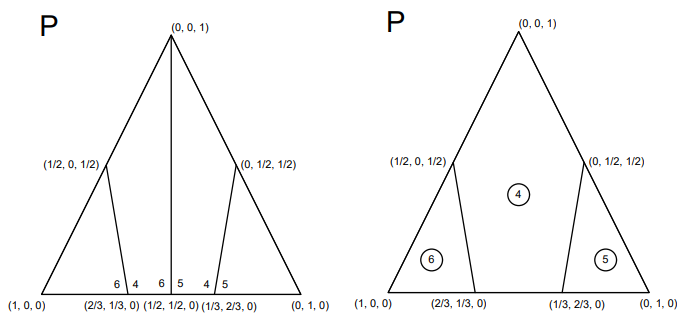
\includegraphics{images/LH1.PNG}
\end{figure}

\noindent
Note that in the second figure the circled numbers are the labels that correspond to the best reply of player 2 in that region.

\noindent
\\
Similarly, for $Q$, we examine, one-by-one, the equations:

\begin{table}[h]
    \centering
    \begin{tabular}{rcl}
        $12q_1 + 2q_2 + 2q_3$ & $=$ & $10q_1 + 8q_2 + 3q_3$ \\
        $12q_1 + 2q_2 + 2q_3$ & $=$ & $9q_1 + 4q_2 + 6q_3$ \\
        $10q_1 + 8q_2 + 3q_3$ & $=$ & $9q_1 + 4q_2 + 6q_3$
    \end{tabular}
\end{table}

\noindent
This gives us the following subdivision:

\begin{figure}[h!]
    \centering
    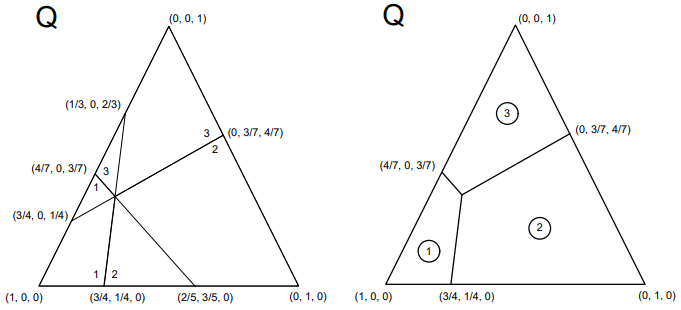
\includegraphics{images/LH2.PNG}
\end{figure}

\noindent
Note that the points on the border between two regions have both labels.

\newpage
\noindent
Recall that actions $p$ for which $p_i = 0$ have label $i$, while actions $q$ for which $q_j = 0$ have label $j$.
This means that, by introducing an artificial vertex $(0, 0, 0)$ outside this triangle, we can label the outside regions as well:

\begin{figure}[h]
    \centering
    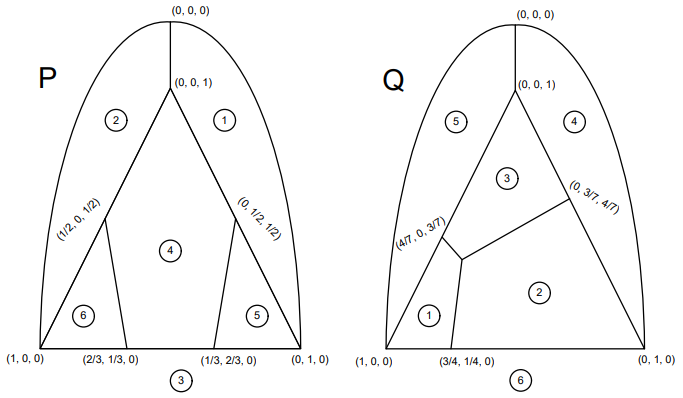
\includegraphics{images/LH3.PNG}
\end{figure}

\noindent
Since we are interested in finding completely labeled pairs of actions, we can replace the coordinates on the vertices by the labels:

\begin{figure}[h]
    \centering
    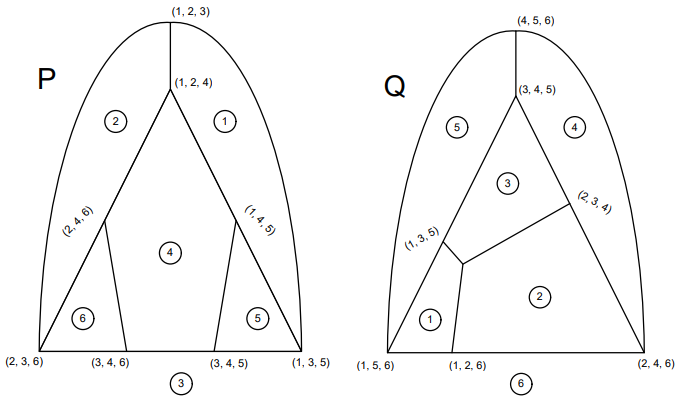
\includegraphics{images/LH4.PNG}
\end{figure}

\noindent
Notice that the artificial pair of actions $(0, 0, 0), (0, 0, 0)$ is a completely labeled pair.
This makes it an interesting starting point for a walk along almost completely labeled pairs of actions.

\newpage
\noindent
If we go on a 1-path, we first move away from the label-1-region in the $P$-graph.
This leads to a new pair of actions where 6 is the double label, thus we have to move away from region 6 in the $Q$-graph.
At the next stop the label 3 is doubled, implying we have to move away from 3 in the $P$-graph.
Next, label 4 is doubled, and we move away from region 4 in the $Q$-graph to find a completely labeled pair!

\begin{figure}[h]
    \centering
    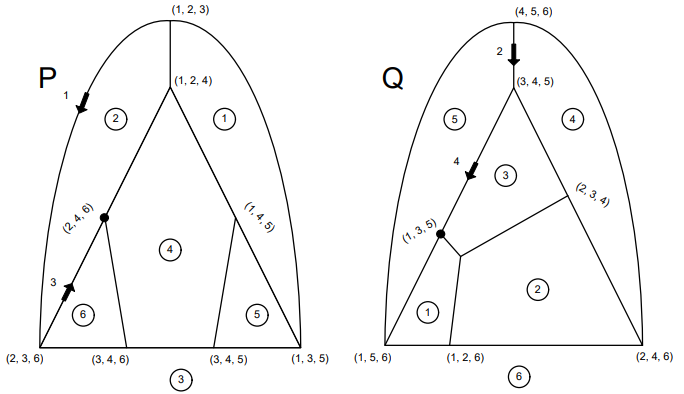
\includegraphics{images/LH5.PNG}
\end{figure}

\noindent
Note that the choice of going on a 1-path is arbitrary.
A different $k$-path could possibly (not necessarily!) lead to a different equilibrium:

\begin{figure}[h]
    \centering
    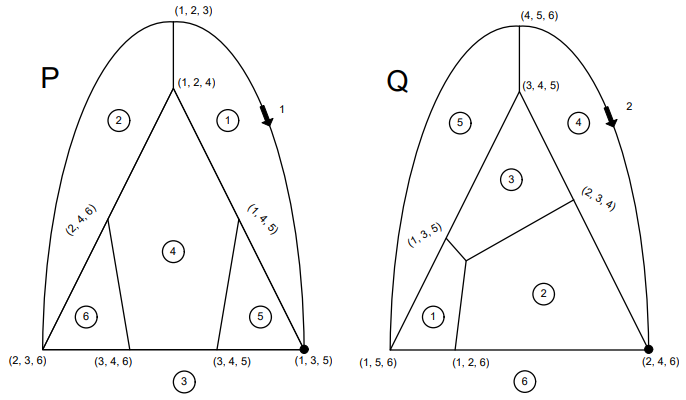
\includegraphics{images/LH6.PNG}
    \caption{A 2-path leading to a different equilibrium.}
\end{figure}

\newpage
\subsection{Tabular Procedure}
We examine the same game $(A, B)$ as before, given by:

\[ A = \begin{pmatrix}
    12 & 2 & 2 \\
    10 & 8 & 3 \\
    9 & 4 & 6
\end{pmatrix} \quad \text{and} \quad
B = \begin{pmatrix}
    2 & 0 & 3 \\
    2 & 3 & 0 \\
    1 & 0 & 0
\end{pmatrix} \]

\noindent
The first step is to create the $P$-tableau (based on $B$) and the $Q$-tableau (based on $A$):

\begin{table}[h]
    \begin{minipage}{.5\linewidth}
        \centering
        \begin{tabular}{c|ccc|ccc|c|c|}
            \cline{2-9}
            \textbf{P} & $p_1$ & $p_2$ & $p_3$ & $s_4$ & $s_5$ & $s_6$ & $-w$ & $=$ \\ \hline
            \multicolumn{1}{|c|}{top} & 1 & 1 & 1 & 0 & 0 & 0 & 0 & 1 \\ \hline
            \multicolumn{1}{|c|}{$s_4$} & 2 & 2 & 1 & 1 & 0 & 0 & 1 & 0 \\
            \multicolumn{1}{|c|}{$s_5$} & 0 & 3 & 0 & 0 & 1 & 0 & 1 & 0 \\
            \multicolumn{1}{|c|}{$s_6$} & 3 & 0 & 0 & 0 & 0 & 1 & 1 & 0 \\ \hline
        \end{tabular}
    \end{minipage}%
    \begin{minipage}{.5\linewidth}
        \centering
        \begin{tabular}{c|ccc|ccc|c|c|}
            \cline{2-9}
            \textbf{Q} & $q_4$ & $q_5$ & $q_6$ & $r_1$ & $r_2$ & $r_3$ & $-u$ & $=$ \\ \hline
            \multicolumn{1}{|c|}{top} & 1 & 1 & 1 & 0 & 0 & 0 & 0 & 1 \\ \hline
            \multicolumn{1}{|c|}{$r_1$} & 12 & 2 & 2 & 1 & 0 & 0 & 1 & 0 \\
            \multicolumn{1}{|c|}{$r_2$} & 10 & 8 & 3 & 0 & 1 & 0 & 1 & 0 \\
            \multicolumn{1}{|c|}{$r_3$} & 9 & 4 & 6 & 0 & 0 & 1 & 1 & 0 \\ \hline
        \end{tabular}
    \end{minipage}
\end{table}

\noindent
Notice how the inner core of the $P$-tableau is the transpose of $B$, and the inner core of the $Q$-tableau is $A$.
These tableaux correspond to $(p_1, p_2, p_3) = (0, 0, 0)$ and $(q_4, q_5, q_6) = (0, 0, 0)$, which implies that we start with a full set of labels $\{ 1, 2, 3, 4, 5, 6 \}$

\noindent
\\
We will again start with a 1-path.
To find what label will be doubled first, we need to find the best reply for player 2 if player 1 plays 1.
In $B$ we can see that action 6 is a best reply for 1.
To remove label 1, we pivot in $P$ on $(\text{top}, p_1)$.
To bring label 6 in, we then pivot in $P$ on $(s_6, -w)$:

\begin{table}[h]
    \centering
    \begin{tabular}{c|ccc|ccc|c|c|}
        \cline{2-9}
        \textbf{P} & $p_1$ & $p_2$ & $p_3$ & $s_4$ & $s_5$ & $s_6$ & $-w$ & $=$ \\ \cline{1-2} \Cline{2pt}{2-2} \cline{3-9}
        \multicolumn{1}{|c|}{top} & \Thickvrule{1} & 1 & 1 & 0 & 0 & 0 & 0 & 1 \\ \cline{1-2} \Cline{2pt}{2-2} \cline{3-9}
        \multicolumn{1}{|c|}{$s_4$} & 2 & 2 & 1 & 1 & 0 & 0 & 1 & 0 \\
        \multicolumn{1}{|c|}{$s_5$} & 0 & 3 & 0 & 0 & 1 & 0 & 1 & 0 \\
        \multicolumn{1}{|c|}{$s_6$} & 3 & 0 & 0 & 0 & 0 & 1 & 1 & 0 \\ \hline
    \end{tabular}
\end{table}

\begin{table}[h]
    \centering
    \begin{tabular}{c|ccc|ccc|c|c|}
        \cline{2-9}
        \textbf{P} & $p_1$ & $p_2$ & $p_3$ & $s_4$ & $s_5$ & $s_6$ & $-w$ & $=$ \\ \hline
        \multicolumn{1}{|c|}{$p_1$} & 1 & 1 & 1 & 0 & 0 & 0 & 0 & 1 \\ \hline
        \multicolumn{1}{|c|}{$s_4$} & 0 & 0 & -1 & 1 & 0 & 0 & 1 & -2 \\
        \multicolumn{1}{|c|}{$s_5$} & 0 & 3 & 0 & 0 & 1 & 0 & 1 & 0 \\ \Cline{2pt}{8-8} 
        \multicolumn{1}{|c|}{$s_6$} & 0 & -3 & -3 & 0 & 0 & 1 & \Thickvrule{1} & -3 \\ \cline{1-8} \Cline{2pt}{8-8} \cline{9-9}
    \end{tabular}
\end{table}

\begin{table}[h!]
    \centering
    \begin{tabular}{c|ccc|ccc|c|c|}
        \cline{2-9}
        \textbf{P} & $p_1$ & $p_2$ & $p_3$ & $s_4$ & $s_5$ & $s_6$ & $-w$ & $=$ \\ \hline
        \multicolumn{1}{|c|}{$p_1$} & 1 & 1 & 1 & 0 & 0 & 0 & 0 & 1 \\ \hline
        \multicolumn{1}{|c|}{$s_4$} & 0 & 3 & 2 & 1 & 0 & -1 & 0 & 1 \\
        \multicolumn{1}{|c|}{$s_5$} & 0 & 6 & 3 & 0 & 1 & -1 & 0 & 3 \\ 
        \multicolumn{1}{|c|}{$-w$} & 0 & -3 & -3 & 0 & 0 & 1 & 1 & -3 \\ \hline
    \end{tabular}
\end{table}

\noindent
\\
This gives us $p = (1, 0, 0)$, $L^1(p) = \{ 2, 3, 6 \}$.

\newpage
\noindent
To move away from $(0, 0, 0)$ in the $Q$-tableau, we need to remove label 6.
If player 2 plays action 6, then, looking at $A$, we see that action 3 is a best reply for player 1.
To remove label 6, we pivot in $Q$ on $(\text{top}, q_6)$.
To bring label 3 in, we then pivot in $Q$ on $(r_3, -u)$:

\begin{table}[h]
    \centering
    \begin{tabular}{c|ccc|ccc|c|c|}
        \cline{2-9}
        \textbf{Q} & $q_4$ & $q_5$ & $q_6$ & $r_1$ & $r_2$ & $r_3$ & $-u$ & $=$ \\ \cline{1-3} \Cline{2pt}{4-4} \cline{5-9}
        \multicolumn{1}{|c|}{top} & 1 & 1 & \Thickvrule{1} & 0 & 0 & 0 & 0 & 1 \\ \cline{1-3} \Cline{2pt}{4-4} \cline{5-9}
        \multicolumn{1}{|c|}{$r_1$} & 12 & 2 & 2 & 1 & 0 & 0 & 1 & 0 \\
        \multicolumn{1}{|c|}{$r_2$} & 10 & 8 & 3 & 0 & 1 & 0 & 1 & 0 \\ 
        \multicolumn{1}{|c|}{$r_3$} & 9 & 4 & 6 & 0 & 0 & 1 & 1 & 0 \\ \hline
    \end{tabular}
\end{table}

\begin{table}[h]
    \centering
    \begin{tabular}{c|ccc|ccc|c|c|}
        \cline{2-9}
        \textbf{Q} & $q_4$ & $q_5$ & $q_6$ & $r_1$ & $r_2$ & $r_3$ & $-u$ & $=$ \\ \hline
        \multicolumn{1}{|c|}{$q_6$} & 1 & 1 & 1 & 0 & 0 & 0 & 0 & 1 \\ \hline
        \multicolumn{1}{|c|}{$r_1$} & 10 & 0 & 0 & 1 & 0 & 0 & 1 & -2 \\
        \multicolumn{1}{|c|}{$r_2$} & 7 & 5 & 0 & 0 & 1 & 0 & 1 & -3 \\ \Cline{2pt}{8-8}
        \multicolumn{1}{|c|}{$r_3$} & 3 & -2 & 0 & 0 & 0 & 1 & \Thickvrule{1} & -6 \\ \cline{1-8} \Cline{2pt}{8-8} \cline{9-9}
    \end{tabular}
\end{table}

\begin{table}[h]
    \centering
    \begin{tabular}{c|ccc|ccc|c|c|}
        \cline{2-9}
        \textbf{Q} & $q_4$ & $q_5$ & $q_6$ & $r_1$ & $r_2$ & $r_3$ & $-u$ & $=$ \\ \hline
        \multicolumn{1}{|c|}{$q_6$} & 1 & 1 & 1 & 0 & 0 & 0 & 0 & 1 \\ \hline
        \multicolumn{1}{|c|}{$r_1$} & 7 & 2 & 0 & 1 & 0 & -1 & 0 & 4 \\
        \multicolumn{1}{|c|}{$r_2$} & 4 & 7 & 0 & 0 & 1 & -1 & 0 & 3 \\
        \multicolumn{1}{|c|}{$-u$} & 3 & -2 & 0 & 0 & 0 & 1 & 1 & -6 \\ \hline
    \end{tabular}
\end{table}

\noindent
This gives us $q = (0, 0, 1)$, $L^2(q) = \{ 3, 4, 5 \}$.

\noindent
\\
We do not need the rows and columns headed by $-u$ and $-w$ any longer, so we can delete these from the tableaux.
This brings us to the following state:

\begin{table}[h!]
    \begin{minipage}{.5\linewidth}
        \centering
        \begin{tabular}{c|ccc|ccc|c|}
            \cline{2-8}
            \textbf{P} & $p_1$ & $p_2$ & $p_3$ & $s_4$ & $s_5$ & $s_6$ & $=$ \\ \hline
            \multicolumn{1}{|c|}{$p_1$} & 1 & 1 & 1 & 0 & 0 & 0 & 1 \\
            \multicolumn{1}{|c|}{$s_4$} & 0 & 3 & 2 & 1 & 0 & -1 & 1 \\
            \multicolumn{1}{|c|}{$s_5$} & 0 & 6 & 3 & 0 & 1 & -1 & 3 \\ \hline
        \end{tabular}\\
        $p = (1, 0, 0)$ \quad $L^1(p) = \{ 2, 3, 6 \}$
    \end{minipage}%
    \begin{minipage}{.5\linewidth}
        \centering
        \begin{tabular}{c|ccc|ccc|c|}
            \cline{2-8}
            \textbf{Q} & $q_4$ & $q_5$ & $q_6$ & $r_1$ & $r_2$ & $r_3$ & $=$ \\ \hline
            \multicolumn{1}{|c|}{$q_6$} & 1 & 1 & 1 & 0 & 0 & 0 & 1 \\
            \multicolumn{1}{|c|}{$r_1$} & 7 & 2 & 0 & 1 & 0 & -1 & 4 \\
            \multicolumn{1}{|c|}{$r_2$} & 4 & 7 & 0 & 0 & 1 & -1 & 3 \\ \hline
        \end{tabular}\\
        $q = (0, 0, 1)$ \quad $L^2(q) = \{ 3, 4, 5 \}$
    \end{minipage}
\end{table}

\noindent
We can see that label 3 appears twice, so the next step is to pivot in the $P$-tableau on column 3.
The pivot row is chosen by maximizing the ratio of the pivot column to the '=' column.
We now alternate pivoting in the $P$-tableau and the $Q$-tableau, each time choosing the pivot column of the double label, until we find a completely labeled pair of actions:

\newpage
\begin{table}[h]
    \centering
    \begin{tabular}{c|ccc|ccc|c|}
        \cline{2-8}
        \textbf{P} & $p_1$ & $p_2$ & $p_3$ & $s_4$ & $s_5$ & $s_6$ & $=$ \\ \hline
        \multicolumn{1}{|c|}{$p_1$} & 1 & 1 & 1 & 0 & 0 & 0 & 1 \\ \Cline{2pt}{4-4}
        \multicolumn{1}{|c|}{$s_4$} & 0 & 3 & \Thickvrule{2} & 1 & 0 & -1 & 1 \\ \Cline{2pt}{4-4}
        \multicolumn{1}{|c|}{$s_5$} & 0 & 6 & 3 & 0 & 1 & -1 & 3 \\ \hline
    \end{tabular}
\end{table}

\begin{table}[h]
    \centering
    \begin{tabular}{c|ccc|ccc|c|}
        \cline{2-8}
        \textbf{P} & $p_1$ & $p_2$ & $p_3$ & $s_4$ & $s_5$ & $s_6$ & $=$ \\ \hline
        \multicolumn{1}{|c|}{$p_1$} & 1 & $-\frac{1}{2}$ & 0 & $-\frac{1}{2}$ & 0 & $\frac{1}{2}$ & $\frac{1}{2}$ \\
        \multicolumn{1}{|c|}{$p_3$} & 0 & $1\frac{1}{2}$ & 1 & $\frac{1}{2}$ & 0 & $-\frac{1}{2}$ & $\frac{1}{2}$ \\
        \multicolumn{1}{|c|}{$s_5$} & 0 & $1\frac{1}{2}$ & 0 & $-1\frac{1}{2}$ & 1 & $\frac{1}{2}$ & $1\frac{1}{2}$ \\ \hline
    \end{tabular}
    \caption*{$p = (\frac{1}{2}, 0, \frac{1}{2})$ \quad $L^1(p) = \{ 2, 4, 6 \}$}
\end{table}

\noindent
4 is the double label, so we pivot in the $Q$-tableau on column 4:

\begin{table}[h]
    \centering
    \begin{tabular}{c|ccc|ccc|c|}
        \cline{2-8}
        \textbf{Q} & $q_4$ & $q_5$ & $q_6$ & $r_1$ & $r_2$ & $r_3$ & $=$ \\ \hline
        \multicolumn{1}{|c|}{$q_6$} & 1 & 1 & 1 & 0 & 0 & 0 & 1 \\ \Cline{2pt}{2-2}
        \multicolumn{1}{|c|}{$r_1$} & \Thickvrule{7} & 2 & 0 & 1 & 0 & -1 & 4 \\ \Cline{2pt}{2-2}
        \multicolumn{1}{|c|}{$r_2$} & 4 & 7 & 0 & 0 & 1 & -1 & 3 \\ \hline
    \end{tabular}
\end{table}

\begin{table}[h!]
    \centering
    \begin{tabular}{c|ccc|ccc|c|}
        \cline{2-8}
        \textbf{Q} & $q_4$ & $q_5$ & $q_6$ & $r_1$ & $r_2$ & $r_3$ & $=$ \\ \hline
        \multicolumn{1}{|c|}{$q_6$} & 0 & $\frac{5}{7}$ & 1 & $-\frac{1}{7}$ & 0 & $\frac{1}{7}$ & $\frac{3}{7}$ \\
        \multicolumn{1}{|c|}{$q_4$} & 1 & $\frac{2}{7}$ & 0 & $\frac{1}{7}$ & 0 & $-\frac{1}{7}$ & $\frac{4}{7}$ \\
        \multicolumn{1}{|c|}{$r_2$} & 0 & $5\frac{6}{7}$ & 0 & $-\frac{4}{7}$ & 1 & $-\frac{3}{7}$ & $\frac{5}{7}$ \\ \hline
    \end{tabular}
    \caption*{$q = (\frac{4}{7}, 0, \frac{3}{7})$ \quad $L^1(p) = \{ 1, 3, 5 \}$}
\end{table}

\noindent
This is a completely labeled pair of actions, so we know $(p, q) = ((\frac{1}{2}, 0, \frac{1}{2}), (\frac{4}{7}, 0, \frac{3}{7}))$ is an equilibrium.

%
% Topic 7 - Stability and Marriage Problems
%
\newpage
\section{Stability and Marriage Problems}
Marriage problems refer to finding a \textbf{stable matching} between males and females, where each individual has a certain preference of the candidates of the other sex.
In this framework, a stable matching is one in which no male and female can be found who prefer each other more than the person they are already matched to, for otherwise the two could get together and be more happy.

\noindent
\\
A marriage problem is described by two preference structures:
one in which each female has ordered all males in order of preference, and one in which each male has ordered all females in order of preference.
Take the following example:

\begin{table}[h]
    \centering
    \begin{tabular}{|c|l|l|l|l|l|}
    \hline
    \backslashbox{\textbf{F}}{\textbf{M}} & \multicolumn{1}{c|}{1} & \multicolumn{1}{c|}{2} & \multicolumn{1}{c|}{3} & \multicolumn{1}{c|}{4} & \multicolumn{1}{c|}{5} \\ \hline
    \textbf{Anny}: & Freddy & Harry & Kenny & Gerry & Lenny \\ \hline
    \textbf{Betty}: & Gerry & Kenny & Freddy & Harry & Lenny \\ \hline
    \textbf{Conny}: & Lenny & Harry & Gerry & Freddy & Kenny \\ \hline
    \textbf{Dolly}: & Harry & Lenny & Freddy & Gerry & Kenny \\ \hline
    \textbf{Emmy}: & Harry & Kenny & Gerry & Lenny & Freddy \\ \hline
    \end{tabular}
\end{table}

\begin{table}[h]
    \centering
    \begin{tabular}{|c|l|l|l|l|l|}
    \hline
    \backslashbox{\textbf{M}}{\textbf{F}} & \multicolumn{1}{c|}{1} & \multicolumn{1}{c|}{2} & \multicolumn{1}{c|}{3} & \multicolumn{1}{c|}{4} & \multicolumn{1}{c|}{5} \\ \hline
    \textbf{Freddy}: & Conny & Betty & Anny & Emmy & Dolly \\ \hline
    \textbf{Gerry}: & Dolly & Anny & Betty & Emmy & Conny \\ \hline
    \textbf{Harry}: & Emmy & Anny & Dolly & Betty & Conny \\ \hline
    \textbf{Kenny}: & Emmy & Conny & Anny & Dolly & Betty \\ \hline
    \textbf{Lenny}: & Emmy & Anny & Betty & Conny & Dolly \\ \hline
    \end{tabular}
\end{table}

\noindent
The problem of finding a stable matching in this setting can be formulated as finding a Nash-equilibrium, as none of the individuals should be able to propose to anyone of the opposite sex who would say "yes".
Looking at the above example, the matching $\{ AH, BK, CG, DF, EL \}$ is not a stable matching, since Anny prefers Freddy to Harry, while Freddy prefers Anny to Dolly.

\noindent
\\
Analyzing the above example in more detail, we can observe that Emmy and Harry should be matched to each other in every stable matching.
Since they like each other best, there is nothing stopping them from finding each other.
This effectively means that we can remove Emmy and Harry from the problem, and solve for the remaining 4 individuals.
Another observation is that since Anny likes Freddy best, we cannot match Freddy to anyone he likes less than Anny.
This means Freddy and Dolly will never be matched together, so we can remove Freddy from Dolly's row, and Dolly from Freddy's row.
Our set of possibilities is becoming more and more clear, but this strategy of manually removing pairings is not very efficient.

\subsection{Gale-Shapley Algorithm}
There is a very simple mathematical procedure to determine a stable matching.
The \textbf{Gale-Shapley algorithm} uses \textbf{repeated proposals}, where the proposals are done either by only males or only females, and always yields the \textbf{optimal stable matching}.

\newpage
\noindent
If in the above example the females were to be the proposing group, then the procedure would develop as follows:

\begin{enumerate}
    \item $A$ proposes to $F$, $F$ accepts as he is still available.
    \item $B$ proposes to $G$, $G$ accepts as he is still available.
    \item $C$ proposes to $L$, $L$ accepts as he is still available.
    \item $D$ proposes to $H$, $H$ accepts as he is still available.
    \item $E$ proposes to $H$, $H$ accepts as he prefers $E$ to $D$.
    \item $D$ proposes to $L$, $L$ refuses as he prefers $C$ to $D$.
    \item $D$ proposes to $F$, $F$ refuses as he prefers $A$ to $D$.
    \item $D$ proposes to $G$, $G$ accepts as he prefers $D$ to $B$.
    \item $B$ proposes to $K$, $K$ accepts as he is still available.
\end{enumerate}

\noindent
After this all females are matched to their best preferred available candidates, therefore the matching $\{ AF, BK, CL, DG, EH \}$ is stable.

\noindent
\\
The Gale-Shapley algorithm can also be used to find stable matchings in situations where the sets of males and females are not of the same size.
Additionally, the algorithm can be used in situations where some individuals would rather stay single than being married to a candidate they do not like.
In this case, we introduce artificial people $(M_1, M_2, ... / W_1, W_2, ...)$ to the preference structures to discriminate between feasible and infeasible candidates.
For example:

\begin{table}[h]
    \begin{minipage}{.45\linewidth}
        \centering
        \begin{tabular}{|c|l|l|l|l|l|l|}
            \hline
            \backslashbox{\textbf{M}}{\textbf{F}} & \multicolumn{1}{c|}{1} & \multicolumn{1}{c|}{2} & \multicolumn{1}{c|}{3} & \multicolumn{1}{c|}{4} & \multicolumn{1}{c|}{5} & \multicolumn{1}{c|}{6} \\ \hline
            \textbf{A}: & F & K & & & & \\ \hline
            \textbf{B}: & G & K & F & L & H & \\ \hline
            \textbf{C}: & L & G & H & & & \\ \hline
            \textbf{D}: & L & F & G & K & & \\ \hline
            \textbf{E}: & H & G & L & & & \\ \hline
        \end{tabular}
    \end{minipage}%
    $\Rightarrow$
    \begin{minipage}{.5\linewidth}
        \centering
        \begin{tabular}{|c|l|l|l|l|l|l|}
            \hline
            \backslashbox{\textbf{M}}{\textbf{F}} & \multicolumn{1}{c|}{1} & \multicolumn{1}{c|}{2} & \multicolumn{1}{c|}{3} & \multicolumn{1}{c|}{4} & \multicolumn{1}{c|}{5} & \multicolumn{1}{c|}{6} \\ \hline
            \textbf{A}: & F & K & $\mathbf{M_1}$ & & & \\ \hline
            \textbf{B}: & G & K & F & L & H & $\mathbf{M_2}$ \\ \hline
            \textbf{C}: & L & G & H & $\mathbf{M_3}$ & & \\ \hline
            \textbf{D}: & L & F & G & K & $\mathbf{M_4}$ & \\ \hline
            \textbf{E}: & H & G & L & $\mathbf{M_5}$ & & \\ \hline
        \end{tabular}
    \end{minipage}
\end{table}

\noindent
Using the Gale-Shapley algorithm you will find at most two stable matchings (depending on which group is the proposing group), but note that there may be more.

\noindent
\\
One other use case of the Gale-Shapley algorithm is to match students $s_1, s_2, ... , s_m$ to universities $U_1, U_2, ... , U_n$.
Each student $s_i$ has a preference over the universities they would like to enter, while each university $U_k$ also has a preference over which students they would like to accept.
In addition to this, each university $U_k$ only has a limited number of spots $n_k$ available.
To use the Gale-Shapley algorithm, we replace each university $U_k$ by $n_k$ copies of $U_k$ ($U_{k,1}, U_{k,2}, ... , U_{k,n_k}$) who are all equally preferred by the students and who all have the same preference over the students.
Even though these matrices can get very large, a stable matching can still be calculated efficiently, as each step of the Gale-Shapley algorithm is very simple.
\end{document}
